\documentclass[11pt,a4paper]{article}
\usepackage[utf8]{inputenc}
\usepackage{fullpage}
\usepackage[T1]{fontenc}
\usepackage{lmodern} % font for the algorithms

%Mathematical language packages
\usepackage{amsmath, amssymb, amsthm, amsfonts, physics, mathtools, mathrsfs, bbm}

\usepackage{enumitem}
\usepackage{xcolor, color}
\usepackage{pdfpages} % to include the front page
\usepackage{mdframed}[framemethod=TikZ] % to draw boxes around algorithms
\usepackage{tikz}

% bibliography
\usepackage[
backend=biber,
style=alphabetic,
]{biblatex}
\addbibresource{bib.bib}

%%%% Theoremstyles
\theoremstyle{plain}
\newtheorem{theorem}{Theorem}[section]
\newtheorem{proposition}[theorem]{Proposition}
\newtheorem{corollary}[theorem]{Corollary}
\newtheorem{claim}[theorem]{Claim}
\newtheorem{lemma}[theorem]{Lemma}
\newtheorem{conjecture}[theorem]{Conjecture}

\theoremstyle{definition}
\newtheorem{definition}[theorem]{Definition}
\newtheorem{algorithm}[theorem]{Algorithm}
\newtheorem{question}[theorem]{Question}
\newtheorem{problem}[theorem]{Problem}

\theoremstyle{remark}
\newtheorem{remark}{Remark}[section]
\newtheorem{remarks}[theorem]{Remarks}
\newtheorem{example}[remark]{Example}
\newtheorem{exercise}[theorem]{Exercise}

% counter of equations resets after each section
\counterwithin{equation}{section}

% custom commands
\newcommand{\R}{\mathbb{R}}
\newcommand{\Q}{\mathbb{Q}}
\newcommand{\C}{\mathbb{C}}
\newcommand{\oQ}{\overline{\mathbb{Q}}}
\newcommand{\Z}{\mathbb{Z}}
\newcommand{\oZ}{\overline{\mathbb{Z}}}
\newcommand{\Oo}{\mathcal{O}}
\newcommand{\B}{\mathcal{B}}
\newcommand{\T}{\mathbb{T}}
\newcommand{\bm}[1]{\boldsymbol{#1}}
\renewcommand{\B}{\bm{B}}
\newcommand{\Bg}{\B_{good}}
\newcommand{\Bb}{\B_{bad}}
\newcommand{\E}{\mathcal{E}}
\newcommand{\p}{\mathfrak{p}}
\newcommand{\q}{\mathfrak{q}}
%\newcommand{\alg}[1]{{\text{\fontfamily{lmss}\selectfont #1}}}
\newcommand{\alg}[1]{\textsf{#1}}
\newcommand{\VF}[1]{\text{Vol}(\mathcal{F(#1)})}
%\newcommand{\prob}[1]{{\fontfamily{cmtt}\selectfont #1}}
\newcommand{\prob}[1]{\texttt{#1}}
\newcommand{\flo}[1]{\lfloor #1 \rfloor}
\newcommand{\round}[1]{\lfloor #1 \rceil}
%\newcommand{\b}{\mathcal{b}}
\newcommand{\Ll}{\mathcal{L}}
\newcommand{\Lld}{\mathcal{L}^{\vee}}
\newcommand{\Rd}{R^{\vee}}
\renewcommand{\mod}{\text{ mod }}
\newcommand{\I}{\mathcal{I}}
\newcommand{\J}{\mathcal{J}}
\newcommand{\Id}{\mathcal{I}^{\vee}}
\newcommand{\D}{\mathcal{D}}
\newcommand{\orc}{\mathfrak{O}}
%\newcommand{\ll}{\mathcal{l}}
%\newcommand{\T}{\mathbb{T}}

\newcommand{\pinar}[1]{{\textcolor{red}{[Pinar: #1]}}}
\newcommand{\marcello}[1]{{\textcolor{red}{[Marcello: #1]}}}
\newcommand{\krzys}[1]{\textcolor{purple}{[Krzys: #1]}}

\usepackage{graphicx} % Required for including pictures
\graphicspath{ {./images/} }
\usepackage{caption}
\usepackage{subcaption} % for images side by side
\usepackage{wrapfig}
%\usepackage{calc} % To reset the counter in the document after title page
%\usepackage{enumitem} % Includes lists

\frenchspacing % No double spacing between sentences
\linespread{1.2} % Set linespace
%\usepackage[a4paper, lmargin=0.1666\paperwidth, rmargin=0.1666\paperwidth, tmargin=0.1111\paperheight, bmargin=0.1111\paperheight]{geometry} %margins
%\usepackage{parskip}
\usepackage[a4paper, lmargin=25mm, rmargin=25mm, tmargin=25mm, bmargin=25mm]{geometry} %margins
\usepackage[all]{nowidow} % Tries to remove widows
\usepackage[protrusion=true,expansion=true]{microtype} % Improves typography, load after fontpackage is selected

\usepackage[pdftex, pdfborder={0 0 0}]{hyperref} % Format links for pdf
\hypersetup{ 	
colorlinks=true,
citecolor=blue,
pdftitle={On ideal lattices in post-quantum cryptography},
pdfauthor={Krzysztof Pudowski},
}

\title{Bachelor Thesis}
\author{Krzysztof Pudowski}
\date{\today}

\begin{document}

\includepdf{front.pdf}

%\maketitle

{\hypersetup{hidelinks} \tableofcontents}

\newpage
\section{Introduction}
\subsection{Why lattices?}
In recent years, the topic of lattice based cryptography (LBC) has seen many developments as an efficient and quantumly secure basis for cryptographic constructions. Starting with Ajtai's seminal work in 1996 \cite{ajtai} on one-way functions that can be reduced to the worst-case problems on lattices we have seen a plethora of new instances like for example NTRU \cite{ntru} or (presented in this paper) LWE \cite{regev} and its ring equivalent \cite{ring-lwe}. We regard them as quantum-resistant because no efficient algorithm is known for solving the underlying hard problems. As the replacement for number-theoretic approaches, lattices have seen the most interest among for example hash-based, code-based or multivariate-quadratic-based implementations. In this paper we focus on the lattice-based approach. We first present some of the older schemes (that have already been broken) and proceed to prove hardness of two other problems. These are the LWE problem and its ring equivalent -- the ring-LWE. Both of them can be reduced to worst-case lattice problems. We present the worst-case reducion for LWE and average-case reduction for ring-LWE.

We build those schemes along another cryptographic construction. This is the fully homomorphic encryption (FHE) which is concerned with performing operations on encrypted data. FHE has been an active area of research since the idea called ``privacy homomorphism'' was presented in \cite{primal} by Rivest, Shamir and Adleman soon after the inception of public-key cryptography. The solution to the problem presented by C. Gentry in his PhD thesis has already seen uses (in its evolved form since 2009) like in for example TNO's implementation for a Zuyderland hospital in their \href{https://eprint.iacr.org/2019/1136.pdf}{Paillier implementation}. In this bachelor thesis we introduce in mathematical terms what FHE is and how we can implement it with the aforementioned (ring-)LWE schemes.
\iffalse
\subsection{Motivation}
include the table from page 16 of \cite{bernstein} of systems broken by quantum computers\\
On the $18^{th}$ of November 2022, a \href{https://www.whitehouse.gov/wp-content/uploads/2022/11/M-23-02-M-Memo-on-Migrating-to-Post-Quantum-Cryptography.pdf}{document} was issued on migrating to post-quantum cryptography.
\fi

\iffalse
This bachelor thesis can be seen as a survey on the recent developments in the LBC and improvements in fully homomorphic cryptographic schemes. Nonetheless, there are few minor contributions that we note here.

Firstly, and most importantly, the introduction of many examples that we hope will be of great help for anyone trying to learn and understand LBC schemes. These include comptutations as well as images and tables that help visualize some key concepts related to Gaussian samples or lattices.

Secondly, we present and explicitly state few results that are otherwise left simply as claims or propositions. These mostly include parts on the algebraic number theory for the Section \ref{ring-lwe} on ring-LWE.
\fi

\subsection{Outline}
The sections in this paper are to be read consecutively with one exception. The Section \ref{ant} on algebraic number theory is mostly useful to prove concepts for ring-LWE from Section \ref{ring-lwe}. If one is not interested in the proofs from this section, it is possible to skip those two since the idea behind ring-LWE is almost identical to the LWE with just minor changes that are not crucial to understand other parts of this paper.

\subsection*{Acknowledgements}
I would like to thank my supervisors, Pınar Kılıçer, for her time and guidance through the areas of algebra and algebraic number theory, as well as Marcello Seri for the project idea and various work-aiding tools. Lastly, I would like to thank my parents and in particular my dad who, long time ago, said ``\textit{You will be thanking me for that later.}'' when urging me to do my mathematics homework. I think this is the right place to say, thank you dad.


\newpage
\section{Background}
\subsection{Notation}
Most of the notation is ``standard'' in the field of number theory and cryptography. Nonetheless, to avoid any misunderstandings and simplify some statements, we will present the notation used throughout the text. Anything that is not mentioned here shall be defined ``on the go'' with definitions and such. \\

\noindent Any scalars $a, t, \beta, \dots$ are represented by non-bold, latin or greek letters.\\
Bold symbols $\bm{v}, \bm{x}, \bm{s}, \dots$ will denote vectors. \\
$\alg{Algorithms}$ will be represented by $\alg{textsf font}$ names such as $\alg{Encrypt}$ or $\alg{Evaluate}$.\\
Traditionally, the symbols $\Z, \Q, \R, \C$ shall represent the sets of integers, rational, real and complex numbers, respectivelly.\\
Additionally, for any real $m \geq 0$, $\flo{m}$ shall denote greatest integer not exceeding $m$, $\round{m} = \flo{m + \frac{1}{2}}$ and $[m]$ is the set $\{1, 2, \dots, \flo{m}\}$.\\
%When the situation demands us to make use of many variables and/or indicies, we will be using Eisenstein notation which is defined as \krzys{fill that in}

\subsection{Lattices}
\subsubsection*{Basic definitions}
We define a \textit{lattice} as a discrete additive subgroup of $\R^n$. Once we fix a basis $\B = (\bm{b}_1, \dots ,\bm{b}_n) \in \R^n$ we can then describe the lattice as
\[ \Lambda = \mathcal{L}(\bm{B}) = \Bigl\{ \sum_i z_i \bm{b}_i : z_i \in \Z \Bigl\}.\]
In other words, $\Lambda$ is the $\Z$-span of the specific basis $\B$.

There are many bases for a lattice (actually, for $n \geq 2$, there are infinitely many as can be proven using a diagonalization argument), some ``better'' than others. This will be the foundation for some of the cryptosystems later like the GGH.

\begin{example}
    The simplest example of a lattice is the $\Z^n$ itself. Taking the standard basis $\B_1 = (\bm{e}_1, \dots, \bm{e}_n)$ we obtain
	\[ \mathcal{L}(\bm{B}_1) = \Bigl\{ \sum_i z_i \bm{e}_i : z_i \in \Z \Bigl\} = \Z^n. \]
\end{example}
More generally, $\Lambda$ is a lattice of rank $m$ in $\R^n$ if it is a rank $m$ free abelian group. Recall that we call a group \textit{free abelian group} of rank $m$ if it can be written as $\Lambda = \Z\beta_1 \oplus \cdots \oplus\Z\beta_m$ with $\beta_1, \dots, \beta_m$ linearly independent over $\R$ where $\oplus$ represents the direct sum. In this paper we will only consider lattices of full rank $n$. 

\begin{remark}
    We can also view the vectors $\bm{b}_i$ as the columns of the matrix $\B \in \R^n \cross \R^n$ in which case, our definition becomes:
    $$\Lambda = \mathcal{L}(B) = \{\bm{Bz} :  \bm{z} \in \Z^n \}.$$
\end{remark}

Reciprocally, any matrix $\bm{B} \in GL_n(\R)$ spans a lattice: the set of all integer linear combinations of its rows.

\begin{example}
\begin{enumerate}
    \item $\mathcal{L} = \begin{pmatrix}
        1 & 0\\
        0 & 1
	\end{pmatrix}$ in which case $\bm{b}_1 = \big(\begin{smallmatrix}
          1\\
          0
	\end{smallmatrix}\big)$ and $\bm{b}_2 = \big(\begin{smallmatrix}
          0\\
          1
        \end{smallmatrix}\big)$
    \item $\mathcal{L} = \{(z_1,z_2) : z_1 + z_2 \text{ is even}\}$
    \item $\mathcal{L} = \begin{pmatrix}
        1/3 & \pi\\
        0 & 21/7
        \end{pmatrix}$
\end{enumerate}
\end{example}

As noted before, the basis of a lattice is not unique. There is one that is particularly interesting to us, namely, the \textit{Hermite Normal Form} (HNF). A basis $\B$ is in HNF if it is upper triangular (or lower triangular - does not matter as long as one is consistent), all elements on the diagonal are strictly positive and any other element $\bm{b}_{i,j}$ satisfies $0 \leq \bm{b}_{i,j} < \bm{b}_{i,i}$.

\subsubsection*{Fundamental Domain}
\begin{definition}[Fundamental Domain] \label{fundamental}
    Let $\mathcal{L}$ be a lattice of dimension $n$ and let $(\bm{b}_1, \dots, \bm{b}_n)$ be a basis for $\mathcal{L}$. The \textit{fundamental domain} (or \textit{fundamental parallelepiped}) for $\mathcal{L}$ corresponding to this basis is the set
    $$ \mathcal{F}(\bm{b}_1, \dots, \bm{b}_n) = \{t_1\bm{b}_1 + \cdots + t_n\bm{b}_n : 0 \leq t_i < 1 \}.$$
\end{definition}

We define the \textit{volume} of $\mathcal{F}(\bm{B})$ as the volume of the corresponding parallelepiped in $\R^n$. The \textit{volume} -- closely connected to the determinant -- plays a very important role in our study which will become evident in later chapters. One of the advantages, of defining the fundamental domain, is that we can formalize the notion of area (or the determinant) of any given lattice. Recall that a lattice is just a countable collection of points and therefore has no volume by itself. This, however, is resolved by introducing the following.

\begin{definition}
    Let $\mathcal{L}$ be a lattice of dimension $n$ and let $\mathcal{F}(\bm{B})$ be a fundamental domain for $\mathcal{L}$ over some basis $\bm{B}$. We define the \textit{determinant} of that lattice as
	\[ \det (\mathcal{L}) = \VF{\bm{B}} = |\det (\bm{B}) | \]
\end{definition}

The next two propositions are arguably the two most fundamental resuls for lattice based cryptography. The first one, states that the $\det (\mathcal{L})$ does not depend on the choice of the basis for that lattice. The second, that our whole ambient space $\R^n$ can be described using only vectors from the lattice and the fundamental domain. We will only give an outline of the proofs for the sake of keeping this section compact. Full proofs, however, can be found in \cite{book}, chapter 6.4.

\begin{lemma}
    The $\det (\mathcal{L})$ of an $n$-dimensional lattice is invariant under the choice of the basis.
\end{lemma}

\begin{proof}[Outline of the proof]
    Let $\bm{B}_1, \bm{B}_2$ be two bases for a lattice $\mathcal{L}$. The crucial part of the proof is to note that any two bases are related by some unimodular matrix $U$ (i.e. a matrix with the determinant of $\pm 1$) s.t. $\bm{B}_1 = U \bm{B}_2$. Then it easily follows that 
	\[| \det (\bm{B}_1) | = \det (\mathcal{L}) = | \det (U \cdot \bm{B}_2) | = | \det(U) | \cdot | \det(\bm{B}_2) | = | \det(\bm{B}_2)| \]
\end{proof}

From now on we will write $\mathcal{F}$ to denote the fundamental domain of the lattice without specifying the basis.

\begin{proposition}
    Let $\mathcal{L} \subset \R^n$ be a lattice of dimension $n$ and let $\mathcal{F}$ be a fundamental domain for $\mathcal{L}$. Then every vector $\bm{v} \in \R^n$ can be written in the form 
    $$\bm{v} = \bm{f} + \bm{t}$$
    for $\bm{f} \in \mathcal{F}$ and $\bm{t} \in \mathcal{L}$ both unique and associated to the original $\bm{v}$.
\end{proposition}

Equivalently, the space $\R^n$ is spanned exactly (without overlap) by shifting the fundamental domain by the vectors from our lattice.
$$ \R^n = \bigcup_{\bm{t} \in \mathcal{L}} \{\bm{f + t} : \bm{f} \in \mathcal{F} \}$$

\begin{remark}
    Sometimes the \textit{fundamental domain} is refered to as a parallelepiped or parallelotope and denoted by caligraphic $\mathcal{P}$. If we take a matrix $\bm{B}$ to represent our lattice $\mathcal{L}$, then $\mathcal{P}_{1/2}(\bm{B}) = \{\bm{x}\bm{B}, \bm{x} \in [-1/2, 1/2]^n \}$ can also represent the (shifted by a half) fundamental domain of $\mathcal{L}$ (like for example in \cite{gentry}).
\end{remark}
\iffalse
We will now present two results that give us an upper bound on the length of the shortest vector in a lattice. This will later on be useful to determine the security and/or correctness of our schemes. These theorems are due to Hermite (1822 - 1901) and Minkowski (1864 - 1909).

\begin{theorem}[Hermite's Theorem]
    Every lattice $\mathcal{L}$ of dimension $n$ contains a nonzero vector $v \in \mathcal{L}$ satisfying
    $$ \norm{v} \leq \sqrt{n} \det(\mathcal{L})^{\frac{1}{n}}.$$
\end{theorem}
\krzys{add minkowski's theorem}\\
\fi
We can also need some notion of the shortest possible vector of a lattice. These will be very useful in the study of the hardness of a given problem.
\begin{definition}
	For a $n$-dimensional lattice $\Ll$, we denote its shortest nonzero vector (also called the \textit{minimum distance}) by $\lambda_1(\Ll)$. Formally
	\[ \lambda_1(\Ll) := \min_{0 \neq \bm{v} \in \Ll} ||\bm{v}|| \]
	More generally, for $1 \leq i \leq n$, the $i$th sucessive minimum of $\Ll$ is
	\[\lambda_i(\Ll) := \inf \{r : \Ll \text{ has $i$ linearly independent vectors of length at most } r \}. \]
\end{definition}
For example, in order to be able to go ``away'' from the lattice $\Ll$ ``out'' into the ambient space $\R^n$ and still be able to return to the original vector, we need to make sure the distance $d$ we travel is at most $\lambda_1(\Ll)/2$. This is for example a requirement in the \prob{BDD} problem where the decoding is \textit{promised}. For the exact definition see Section \ref{hardness}.

Aditionally, most of the problems used in this paper are the \textit{approximate} versions to some varying constant usually called $\gamma$. As we will see later, $\gamma$ very often depends on $\lambda_1(\Ll)$ which roughly measures how ``strict'' or ``precise'' we can make our problem. This will be made explicing in the Section \ref{hardness} on the hardness and complexity theory.

\paragraph{Dual}
\begin{definition}[Dual]
    For a lattice $\Ll \subset \R^n$ its $\Z$\textit{-dual} is
    \[ \Lld = \{ y \in \R^n : \langle y,\Ll \rangle \subseteq \Z \}.\]
\end{definition}

We simply require that the elements of the dual to be precisely those vectors, that yield an integer when ``multiplied'' with an element of our lattice. Note that this is different from our standard definition of a dual. Namely, it is not the orthogonal compliment of our starting space, i.e. not all of the elements of the dual have 0 dot product against the vectors of the lattice.

\begin{example}\label{ld-ex}
    Take $\mathcal{L}= \Z 
        \big(\begin{smallmatrix} 1\\2 \end{smallmatrix}\big) + 
        \Z \big(\begin{smallmatrix} 0\\ 1 \end{smallmatrix}\big)$.
        To calculate the dual of $\mathcal{L}$ we need our $y = \big(\begin{smallmatrix}
          a\\b\end{smallmatrix}\big)$ elements to satisfy $a +2b \in \Z$ and $b \in \Z$ which is equivalent to asking $a \in (1/2)\Z$ and so $\mathcal{L}^{\vee} = \big(\begin{smallmatrix}
          1/2\\0
        \end{smallmatrix}\big)\Z + \big(\begin{smallmatrix}
          0\\1
        \end{smallmatrix}\big) \Z$
        See Figure \ref{lattices} where the red vectors represent the basis.
\end{example}

Note that $\mathcal{L}^{\vee}$ is itself a lattice of the same dimension. One can imagine the dual as the original lattice ``flipped'' in the sence that the shortes element becomes the longest and vice versa.
\begin{figure}[ht]
    \caption{Lattice $\Ll$ from example \ref{ld-ex} and its dual.}
        \label{lattices}
        \centering
        \begin{subfigure}{.5\textwidth} 
                \centering
                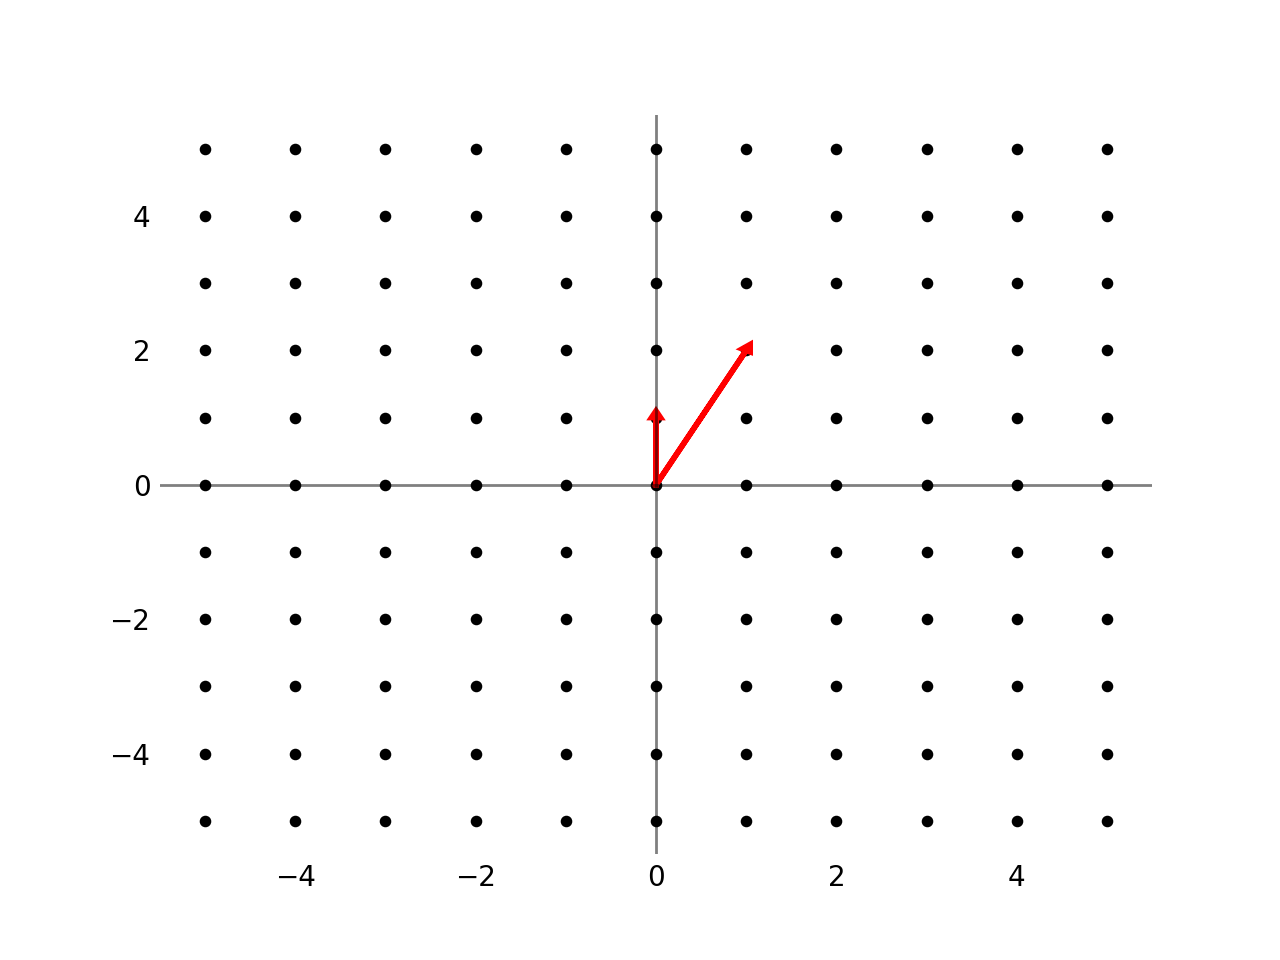
\includegraphics[scale=0.5]{lattice.png}
                \caption{$\Ll$}
        \end{subfigure}%
        \begin{subfigure}{.5\textwidth}
                \centering
                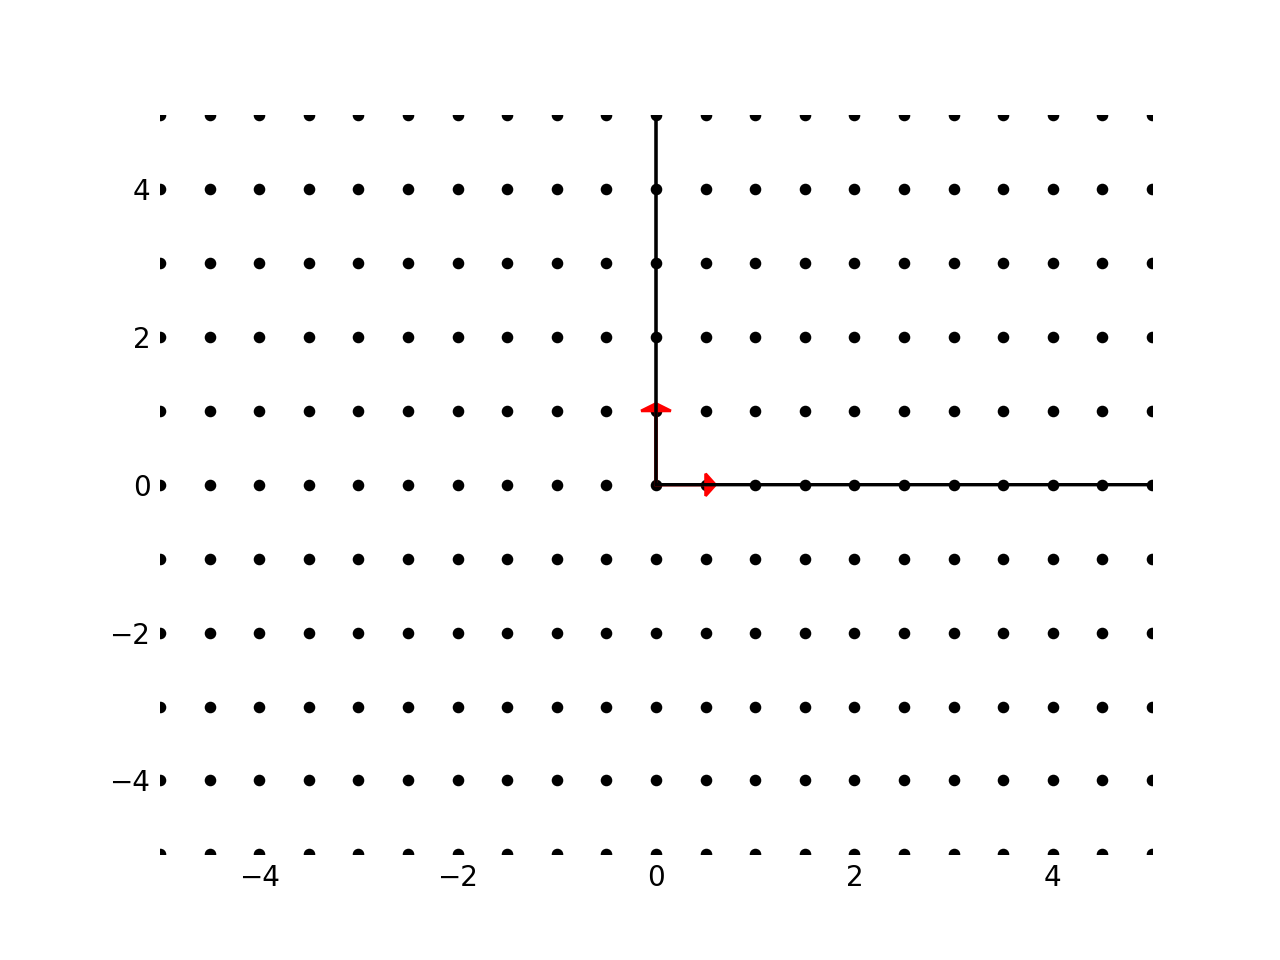
\includegraphics[scale=0.5]{lattice-d.png}
                \caption{$\Lld$}
        \end{subfigure}
\end{figure}

\subsection{Algebraic Number Theory}\label{ant}
Algebraic number theory is the study of \textit{number fields}, \textit{rings of integers} and \textit{finite fields}. In this section we will provide all the necessary background needed to understand and verify the results presented in the cryptographic schemes later in the text. Most results will be stated without proof however all of them can be found in the books like \cite{algebra} and \cite{ribenboim}.

\subsubsection*{Number Fields}
A \textit{number field} is defined as a subfield of $\oQ$ having finite dimension as a vector space over the rationals $\Q$. The \textit{degree} of a number field $K$ is defined as the dimension of $K$ over $\Q$ and when not stated otherwise, will be denoted by $n$. There exists a monic irreducible polynomial\footnote{Recall that we call polynomial monic if its leading coefficient is 1. It is an irreducible polynomial if it is irreducible as an element of the polynomial ring $\Q[x]$.} $f \in \Q[x]$ such that $K \cong \Q[x]/(f )$. In fact, every monic and irreducible polynomial in $\Q[x]$ defines a number field via such isomorphism.

\begin{definition}[Algebraic integer]
    An element $\alpha \in \C$ is an \textit{algebraic integer} if and only if, it is a root of some monic polynomial in $\Z[x]$.
\end{definition}
In fact, the set of \textit{algebraic integers} forms a ring.

\begin{definition}[Ring of Integers]
We define the \textit{ring of integers} (sometimes also called \textit{maximal order}) $\Oo_K$ of a number field $K$ as the intersection:
$$
  \Oo_K = K \cap \overline{\Z} = \{x \in K : \text{ $x$ is an algebraic integer}\}.
$$
\end{definition}

\begin{example}
    The field $K = \Q$ is a number field of degree 1. Its ring of integers is, as one can guess, the ordinary integers $\Z$.
\end{example}

\begin{example}\label{z-basis}
	The ring of Gaussian integers $\Z[\sqrt{-1}] = \{a+b\sqrt{-1}\, : \, a,b \in \Z \}$ is the ring of integers of $K = \Q(\sqrt{-1}) = \{a + b\sqrt{-1} \, : \, a,b\in \Q\}$ which has degree 2 since $x^2+1$ is the minimal (and irreducible) polynomial of $\sqrt{-1}$ over $\Q$. Note that $\Oo_K$ is spanned by $\{1, \sqrt{-1} \}$.
\end{example}

As another example, we can make a following statement about the ring of integers of a quadratic extension of rationals (real quadratic field).
\begin{lemma}
     Let $d \in \Z$ be a square-free integer. For the field $K = \Q(\sqrt{d})$, its ring of integers is 
     \[ \Oo_K = 
	 \begin{cases} 
	     \Z[\sqrt{d}] & \text{if $d \equiv 2, 3 \mod 4$}, \\
	     \Z[(1 + \sqrt{d})/2] & \text{otherwise}.
     	 \end{cases}
     \]
\end{lemma}

\begin{proof}
	Take $d \equiv 1 \mod 4$ square-free. \pinar{if you dont have time to finish the proof give a reference.}
\end{proof}
For example for $K = \Q(\sqrt{5})$ its ring of integers is $\Oo_K = \Z[(1 + \sqrt{5})/2]$. 
\begin{remark}\label{monogenic}
	What is worth noting here, is that for a number field $\Q(\alpha)$ for some $\alpha \in \oQ$, the ring of integers is not necessarily the $\Z[\alpha]$. Instead, $\Z[\alpha]$ is what's called an \textit{order} in $\Oo_K$. We will not consider them in general here because they are not relevant for our study as motivated in the next subsection. In general, a field $K = \Q(\alpha)$ such that $\Oo_K = \Z[\alpha]$ is called a \textit{monogenic} field or a \textit{simple algebraic extension}. For more details on orders, look at for example Chapter 5 of \cite{stein}.
\end{remark}

Recall that an ideal $\I$ of some ring $R$ is an additive subgroup of $R$ (if $x,y \in \I$ then $x-y \in \I$) and closed under multiplication of the elements in $R$ ($x \in \I$ implies $r \cdot x \in \I$ for any $r \in R$). We call an ideal in a ring of integers an \textit{integral ideal}.

One useful property of the integers we would like to preserve is the unique prime decomposition of its elements as stated in the Fundamental Theorem of Algebra. As the name might suggest\footnote{As stated on p.34 in \cite{stein} ``\textit{...it is this unique factorization that initially motivated the introduction of rings of integers of number fields over a century ago''}.}, the ring of integers has a property analogous to such decompositions. Namely, that every nonzero proper ideal factors uniquely into prime ideals. Such ring in general is called a \textit{Dedekind domain}.

More precisely, take $D$ to be a Dedekind domain (for example $\Oo_K$) and $\I \subset D$ a nonzero ideal (and also not an empty set). Then $\I$ factorizes uniquely (up to ordering) into prime ideals $\I = \p_1^{e_1} \p_2^{e_2} \ldots \p_r^{e_r}$ where each $e_i$ is an integer and each $\p_i$ is prime. Additionally it can be shown that in a Dedekind domain, every prime ideal $\p$ is also \textit{maximal}. This in turn implies that $D/\p$ is a finite field of order equal to the index of $|D /\p|$ as an additive subgroup of $D$.

As mentioned before, it is not in general true that $\Oo_K$ is a principal ideal domain. To mimic the notion of divisibility we will associate the elements of $\Oo_K$ with \textit{fractional ideals}.
\begin{definition}[Fractional ideal]
	A \textit{fractional} ideal of $\Oo_K$ is an ideal $\I$ of $K$ such that there exists some $\alpha \in \Oo_K$ such that $\alpha \cdot \I \subseteq \Oo_K$.
\end{definition}
The fractional ideals are genuine ideals of the field $K$ that were ``divided by something'', hence the name \textit{fractional}. We can also define their inverses as the set
\[ \I^{-1} = \{ \alpha \in K : \alpha \cdot \I \subset \Oo_K \}. \]

Therefore, the set of nonzero fractional ideals of $\Oo_K$ forms a group under multiplication with multiplication defined as $(\alpha \I)(\beta \J) := \alpha \beta \, \I \J$ and $\Oo_K$ itself acting as the identity element. %Since any (fractional) ideal $\I$ factorizes uniquely into prime ideals

\subsubsection*{Embeddings in $\C$} 
Let $K = \Q(\alpha)$ be a number field of degree $n$ for a root $\alpha$ of some irreducible $f \in \Q[x]$. It can be shown, that there are exactly $n$ embeddings (injective ring homomorphisms) of $K$ in $\C$. This can be shown noting that since $\Q$ has characteristic 0, all of the roots of $f$ over $K$ must be distinct. Therefore $\alpha$ can only be sent to any one of its $n$ conjugates over $\Q$. Each conjugate $\beta$ determines a unique embedding $\sigma_i: K \rightarrow \C$ and every embedding must arise in this way since $\alpha$ must be sent to one of its conjugates.

\begin{example}
    The quadratic field $\Q[\sqrt{d}]$, $d$ squarefree, has two embeddings in $\C$: The identity mapping, and also the one which sends $a + b\sqrt{d}$ to $a - b\sqrt{d}$ ($a$, $b$ $\in \Q$), since $\sqrt{d}$ and $-\sqrt{d}$ are the two conjugates of $\sqrt{d}$.
\end{example}
 
%As noted, we have many embeddings in $\C^n$. The simplest case could be the na\"ive coefficient embedding. Simply take an element of our number field $\alpha \in K = \Q[x]/(f)$ seen as a polynomial ring and map each of the coefficients $\alpha_i$ into the corresponding spot of the $\C^n$ vector. Although easy to picture, we will instead almost exclusively be using the \textit{canonical embedding} defined as follows.

\begin{definition}[Canonical embedding]
	Let $K = \Q(\alpha)$ be a simple algebraic extension (generated by just $\alpha$) of $\Q$ of degree $n$. Let $f(x)$ be the minimal polynomial of $\alpha$. Denote by $\sigma_i : K \rightarrow K$ the $\Q-$automorphism such that $\sigma_i(\alpha) = \alpha_i$ where $\alpha := \alpha_1$ and $\alpha_i$ are the roots of $f(x)$. The \textit{canonical embedding} $\sigma$ is defined as
	\[ \sigma : K \rightarrow \C^n, \; \; \; \alpha \mapsto  (\sigma_1(\alpha), \sigma_2(\alpha), \ldots, \sigma_n(\alpha)). \]
\end{definition}

\begin{example}
    For $K = \Q(\sqrt{5})$ we have two embeddings $a+b\sqrt{5} \mapsto a \pm b\sqrt{5}$ and so the cannonical embedding is given by
	\[ a + b\sqrt{5} \mapsto (a + b\sqrt{5},\, a - b\sqrt{5}). \]
\end{example}

One last thing we will need to introduce are the \textit{trace} of some field $K$.

\begin{definition}
	Let $K$ be a number field with $n = [K:\Q]$ and let $\sigma_1, \sigma_2, \ldots, \sigma_n$ denote the embeddings of $K$ in $\C$ just like above. For $\alpha \in K$ we define the \textit{trace} as
	\[ \Tr_{K/\Q}(\alpha) = \sum_{i \in [n]} \sigma_i(\alpha). \]
\end{definition}


\subsubsection*{Cyclotomic fields}
One particularly handy family of polynomials are the \textit{cyclotomic polynomials}. As defined momentarily, they are the minimal polynomials of the primitive roots of unity which poses many interesting algebraic properties. They also turn out to be much easier to compute and in general perform computational operations over, in contrast to most other polynomials.

\begin{definition}[Roots of unity]\label{r-of-1}
    Given a field $K$ and a positive integer $n$, an element $\zeta \in K$ is called \textit{primitive $n$-th root of unity} if $\zeta$ has order $n$ in the multiplicative group $K^{\cross}$. In other words, $\zeta^n = 1$ and $\zeta^k \neq 1$ for $1 \leq k < n$. 
\end{definition}
It is also true that all $\zeta^k$ for $1 \leq k < n$ and $\gcd(k,n) = 1$ are conjugates of $\zeta$. It follows that $\Q(\zeta)$ has degree $\varphi(n)$ over $\Q$. This leads us to the following proposition. Recall that the Galois group Gal$(K/\Q)$ of a finite extension of degree $n$ of $K$ over $\Q$ (or any other field for that matter) is the group of all $\Q-$automorphism. That is, Gal$(K/\Q)$ consists of maps $\tau : K \rightarrow K$ that fix $\Q$ elementwise. As a result the image of $\Q$ under $\tau$ is still $\Q$. 
\begin{proposition}[p. 13 in \cite{algebra}]\label{galois}
	The Galois group of $K = \Q(\zeta_n)$ over $\Q$ is isomorphic to the multiplicative group of integers$\mod n$
	\[ \Z_n^* = \{ k : 1 \leq k < n, \; \gcd(k,n) = 1 \}. \]
	For each $k \in \Z_n^*$ the corresponding automorphism in Gal$(K/\Q)$ sends $\zeta$ to $\zeta^k$.
\end{proposition}

The minimal polynomial $\Phi_n$ of $\zeta$ over $\Q$ is called the $n$-th cyclotomic polynomial. Formally we define it as 
\[ \Phi_n(x) = \prod_{\substack{\gcd(k,n) = 1 \\ 1 \leq k < n}} \bigg( x - \zeta^k \bigg) = \prod_{\substack{\gcd(k,n) = 1 \\ 1 \leq k < n}} \bigg( x - e^{2\pi k \sqrt{-1}/n} \bigg) \in \Z[x]. \]

The following equality is very useful for computing the polynomial itself:
\begin{equation}\label{comp_cycl} 
	\Phi_n(x) = (x^n - 1) \bigg/ \prod_{\substack{d | n\\ 1 \leq d < n}} \Phi_d(x) 
\end{equation}
\begin{example}
	To find $\Phi_8(x)$, we can use equation \ref{comp_cycl} to first precompute:
  \begin{align*}
	  & \Phi_1(x) = x - 1 \\
	  & \Phi_2(x) = x^2-1\Big/\Phi_1(x) = \frac{x^2 - 1}{x-1} = x+1 \\
	  & \Phi_4(x) = x^4-1\Big/\Phi_1(x)\cdot \Phi_2(x) = \frac{x^4-1}{(x-1)(x+1)} = x^2 + 1
  \end{align*}
	  And use it one more time to find:
	  \begin{align*}
		  \Phi_8(x) = \; & (x^8 - 1) \Big/ \prod_{{d | 4}} \Phi_d(x) = \Phi_1(x) \cdot \Phi_2(x) \cdot \Phi_4(x) \\
		  = \; & (x^8 - 1) \Big/(x-1)(x+1)(x^2+1) \\
		  = \; & (x^4+1)\cdot (x^2+1)(x+1)(x-1) \Big/(x^2+1)(x+1)(x-1) \\
		  = \; & x^4 +1,
	  \end{align*}
	  as desired.
\end{example}
As a useful corollary of the equation \ref{comp_cycl}, we can prove that for $n$ a power of 2, $n = 2^k$ for some $k \geq 1$, the cyclotomic polynomial $\Phi_n(x)$ is of the form $x^{2^{k - 1}} + 1$.
\begin{corollary}\label{2k-cycl}
  Let $n= 2^k$ for some $k \in \Z_{> 0}$. Then $\Phi_n(x) = x^{2^{k-1}} + 1$.
\end{corollary}
\begin{proof}
	We prove this by induction. We first check that indeed $\Phi_2(x) = x+1$. For the inductive step, assume that we have $\Phi_n(x) = x^{2^{k-1}} + 1$ for some $n = 2^k$. Then it is not difficult to see that $x^{2^k} -1$ ``splits'' as 
	\begin{align*}
		x^{2^k} = & (x^{2^{k-1}} + 1)(x^{2^{k-1}} - 1) \\
		= & (x^{2^{k-1}} + 1)(x^{2^{k-2}} + 1) \cdot \ldots \cdot (x+1)(x-1) \\
		= & (x^{2^{k-1}} + 1) \cdot \Phi_{2^{k-1}}(x) \cdot \ldots \cdot \Phi_2(x) \cdot \Phi_1(x) \\
		= & (x^{2^{k-1}} + 1) \cdot \prod_{d | n} \Phi_d(x)
	\end{align*}
	and so the equation \ref{comp_cycl} becomes
	\begin{align*}
		\Phi_n(x) = & (x^n - 1) \Big/ \prod_{d|n} \Phi_d(x) \\
		= & (x^{2^{k-1}} + 1) \cdot \prod_{d|n} \Phi_d(x) \Big/ \prod_{d|n} \Phi_d(x)\\
		= & x^{2^{k-1}} + 1
	\end{align*}
\end{proof}

As mentioned in Remark \ref{monogenic}, rings of integers are usually not generated by a single element. However, one very useful feature of cyclotomic fields is that their ring of integers is actually just $\Z[\zeta]$. That is -- $\Oo_K = \Z[\zeta]$ for $K = \Q(\zeta)$ and $\zeta$ is some $n$-th root of unity. This greately simplifies the approach in proving some of the results later in this paper as we will only need to look at what happens with $\zeta$ instead of all other generators.

\begin{proposition}\label{cycl-ok}
	The ring of integers of a cyclotomic number field $K = \Q[x]/\Phi_m(x) \cong \Q(\zeta)$ is $\Oo_K = \Z[\zeta]$. Additionally, if $n = \varphi(m)$ is the degree of $K$, then $\Z[\zeta]$ is generated by $\{1, \zeta, \zeta^2, \dots, \zeta^{n-1} \}$.
\end{proposition}

\begin{example}
		Similarly, for $K = \Q(\zeta_5) = \Q[x]/(x^4 +x^3 +x^2+x +1)$, we have four embeddings. These are precisely $\sigma_i(\zeta) = \zeta^i$ and now the canonical embedding maps $a + b\zeta + c\zeta^2 + d\zeta^3$ to
	\begin{align*}
		\begin{pmatrix}
		a + b\zeta + c\zeta^2 +d \zeta^3 \\
		a + b\zeta^2 + c\zeta^4 +d \zeta^6 \\
		a + b\zeta^3 + c\zeta^6 +d \zeta^9 \\
		a + b\zeta^4 + c\zeta^8 +d \zeta^{12}
		\end{pmatrix} = \begin{pmatrix}
		a + b\zeta + c\zeta^2 + d\zeta^3 \\
		a + b\zeta^2 + c\zeta^4 + d\zeta \\ 
		a + b\zeta^3 + c\zeta + d\zeta^4 \\
		a + b\zeta^4 + c\zeta^3 + d\zeta^2
		\end{pmatrix} = \\
		\begin{pmatrix}
		a + b\zeta + c\zeta^2 + d\zeta^3 \\
		a + d\zeta + b\zeta^2 + e\zeta^3 \\
		a + c\zeta + e\zeta^2 + b\zeta^3  \\
		a + e\zeta + d\zeta^2 + c\zeta^3 
		\end{pmatrix} = \begin{pmatrix} sth here
	\end{pmatrix}
	\end{align*}
	\krzys{i feel like i should get something nice but cant figure it our, its probs the $\zeta^4$}
\end{example}

In order to make $\sigma$ a ring homomorphism, we define the addition and multiplication in $\C^n$ to be coordinate-wise (all the conditions for a ring structure are immediate to see when written down because the $\C$ itself is a ring).

Another very handy property of the cyclotomic fields is that for $n > 3$, the $n$-th cyclotomic field has $\varphi(n)$ embeddings in $\C$. These are precisely the $\varphi(n)$ automorphisms where $\sigma_i(\zeta) = \zeta^i$ is simply the conjugation of the generator. Therefore $K$ has only complex embeddings and we call such field a CM-field. Since the $\Q$-automorphisms map $\zeta$ to one of its conjugates, it is easy to see that any automorphism $\tau_k : K \rightarrow K$ mapping $\tau_k(\zeta) = \zeta^k$ simply permutes the coordinates of the canonical embedding. More precisely, $\sigma_i(\tau_k(\zeta)) = \sigma_i(\zeta^k) = \zeta^{ik}$ for all $i,k \in \Z_{\varphi(n)}^*$. Hence $\sigma \circ \tau_k$ is just a permutation of the coordinates.

\subsubsection*{Ideal lattices}
Let us now get back to the topic of lattices for a moment and try to connect those two subjects a bit. Although not shown in this paper, we note that each element of $\Oo_K$ can be expressed as an integer linear combination of some basis $\bm{\mathcal{B}} = \{\beta_1, \beta_2, \ldots, \beta_n \} \subset \Oo_K$ (see the Exercise \ref{z-basis} as a simple case.). The set $\bm{\mathcal{B}}$ is also called the \textit{integral basis} of $\Oo_K$ and is also a basis for $K$ as $\Q$-vector space. Now recall from the beginning of the previous section that any lattice can be defined as the $\Z$-span of some specific basis $\mathcal{\bm{B}} \subset \R^n$. Analogously, we can define a lattice for any number field $K$.

\begin{definition}
	In a number field $K$ of degree $n$, a lattice in $K$ is the $\Z$-span of a $\Q$-basis of~$K$.
\end{definition}
Examples of lattices in $K$ include the ring of integers $\Oo_K$, fractional ideals of $\Oo_K$ and orders in $K$. By the unique decomposition, for any (fractional) ideal in $\Oo_K$, it can be shown that any such ideal is a free abelian group and is spanned by some $\Z$-basis $\{\beta_1, \beta_2, \ldots, \beta_n \}$. Therefore, under the canonical embedding $\sigma$, the ideal yields a rank-$n$ \textit{ideal lattice} with basis $\{\sigma(\beta_1), \ldots \sigma(\beta_n) \} \subset \C^n$. For convenience, we will often associate $\I$ with its embedding in $\C^n$ and talk for example about the shortest vector $\lambda_1(\I)$ of an ideal.

Analogously to the lattices in $\R^n$, we can define duals of lattices in $K$.
\begin{definition}
	Let $\Ll$ be a lattice in $K$. Its \textit{dual lattice} is
	\[\Lld = \{ \alpha \in K : \Tr_{K/\Q}(\alpha \Ll) \subset \Z \}.\]
\end{definition}
Imagine now, that we have some basis $\{1, \alpha, \ldots, \alpha^{n-1} \}$ for a number field $K = \Q(\alpha)$. If, in addition, $\alpha \in \Oo_K$ then the dual basis is characterized by the following proposition (this is special case of Theorem 3.7 in \cite{conrad}).
\begin{proposition}\label{d-basis}
	Let $K = \Q(\alpha)$ and let $f(x)$ be the minimal polynomial of $\alpha$ in $\Q[x]$. Then the dual basis to $\{1, \alpha, \ldots, \alpha^{n-1} \}$ (relative to the trace) is given by:
\[\biggl\{ \frac{1}{f'(\alpha)}, \frac{\alpha}{f'(\alpha)}, \ldots, \frac{\alpha^{n-1}}{f'(\alpha)} \biggr\} . \]
\end{proposition}
The lattice we will be most interested with is the ring of integers $\Oo_K$ itself. What can we say about $\Ood_K = \{ \alpha \in K : \Tr_{K/\Q}(\alpha \Oo_K) \subset \Z \}$? Firstly, it is the largest fractional ideal in $K$ whose elements all have trace in $\Z$ -- \cite{conrad}. The most important result for us however is how the dual of ring of integers ``controls'' every other fractional ideal $\I$.
\begin{proposition}
	For a fractional ideal $\I$ in K, $\I^{\vee}$ is a fractional ideal and $\I^{\vee} = \I^{-1} \Ood_K$.
\end{proposition}
\begin{remark}
The inverse of $\Ood_K$ is called the \textit{different ideal} and was first introduced by Dedekind in 1882 \cite{dedekind}. It has many interesting properties and we refer the curious reader to \cite{conrad} for more details about it as we will not mention anything else about it here.
\end{remark}








\subsection{Complexity Theory and Hard Problems} \label{hardness}
When talking about cryptography, we cannot avoid talking about algorithms since an encryption scheme is simply that, an instruction on how to encode sensitive data. We will thus require some terminology from computational complexity theory -- a field on the overlap of computer science and mathematics -- and cryptography. The problems the former field is concerned with are those of the time and space required for solving computational problems. Most of the time, the goal of the study is to prove the lower bound on the resources required to solve a problem using the best know algorithm. For example, how long does it take to find a factorization of a large composite number. The concern of the later -- cryptography -- is how to efficiently share secrets. The goal of this section is to give an overview of few parts of both fields which we will be using throughout the paper. 

\subsubsection*{Complexity theory}
We begin with necessary terminology. Throughout this section, $n$ shall denote the ``size'' of the input to the algorithm. Here the word ``size'' could mean many things like for example the bit-length of a number or its value in the base 10 representation.

In order to represent the time or space required to solve the problem, most of the time we will use the asymptotic notation of which the ``big-O'' is the most common. For any function $f$ and $g$ of some variable $n$, we say that $f(x) \in O(g(n))$ if there exists some constant $M > 0$ and $n_0$ such that $f(n) \leq Mg(n)$ for all $n \geq n_0$. Roughly speaking, the function $g$ will eventually ``grows faster'' than $f$. Variations on this notations include:

\begin{itemize}
	\item $f \in o(g)$ -- just like $O(g)$ but the inequality holds for all constants $M$. This provides more strict bounds as for example $2n = o(n^2)$ but $2n^2 \neq o(n^2)$ contrary to $2n^2 = O(n^2)$ (as well as $2n = O(n^2)$).
	\item The ``inverse'' of the small $o$ is $\omega$. Formally $f \in \omega(g)$ if for any $M$ there exists $n_0$ such that $f(n) \geq Mg(n)$ for all $n > n_0$. We call it the inverse of $o$ because $f(n) = o(g(n))$ if and only if $g(n) = \omega(f(n))$.
	\item $\tilde{O}(n) = O(n \ln n)$. That is, $\tilde{O}$ hides the logarithmic factors. For example, the FFT (Fast Fourier Transform) computes the discrete Fourier transform in time $O(n \ln n) = \tilde{O}(n)$ for a sequence of length $n$ and Shor's algorithm computes factorization of $n$-bit integer in time $O(n^2 \ln(n) \ln(\ln(n))) = \tilde{O}(n^2)$.
\end{itemize}

We will very often be talking about the ``efficiency'' of an algorithm. Intuitively, we want our procedure to run in a time reasonably proportional to the size of input. The consensus in the academia is to define ``efficient'' as running in polynomial time $\alg{poly}(n)$\footnote{As elegantly stated by Christos Papadimitiou: \textit{``It should not come as a surprise that our choice of polynomial algorithms as the mathematical concept that is supposed to capture the informal notion of ‘practically efficient computation’ is open to criticism from all sides. [$\ldots$] Ultimately, our argument for our choice must be this: Adopting polynomial worst-case performance as our criterion of efficiency results in an elegant and useful theory that says something meaningful about practical computation, and would be impossible without this simplification.''}}. More precisely, 
\begin{definition}
	An algorithm $A(n)$ is \prob{efficient} if there exists a polynomial $p(\cdot)$ such that the computation of $A(n)$ terminates within at most $p(n)$ steps.
\end{definition}
To encapsulate the notion of ``small'' or ``insignificant'', we define a \prob{negligible} amount in $n$ as an amount that is asymptotically smaller than $n^{-c}$ for any constant $c > 0$. More precisely, 
\begin{definition}\label{negl}
    $f (n)$ is a \prob{negligible} function in $n$ if 
	\[\lim_{n \to \infty}n^{-c} \cdot f (n) = 0\]
	for any $c > 0$.
\end{definition}

\subsubsection*{Hard problems}
The basis for modern day cryptography are so called ``hard problems'' of which usage was first formally introduced by S. Goldwasser and S.Micali in \cite{prob-cryp}. These are computational problems for which we do not know any efficient algorithm for (so far). The current approach to cryptography is to assume that some given problem is ``difficult'' to solve and then to prove that the scheme is secure given this assumption. The approach for the proof is to \textit{reduce} our scheme to the one we assume is hard. We proceed by showing how, an adversary, which is able to efficiently solve (or break) our scheme, is able to solve the underlying problem. We call such procedure a \textit{reduction} algorithm. For example, the basis for $\alg{RSA}$ is our inability to efficiently solve the factorization problem.
\begin{definition}[\prob{FACTORIZE}]
	Given a composite integer $n$ and $l < n$, find a non-trivial factor of $n$ less than $l$.
\end{definition}
In their paper \cite{rsa}, Rivest et. al. showed that ``\textit{[$\ldots$] breaking our system is at least as difficult as factoring $n$.''} which is precisely the idea behind a reduction algorithm. Another example of a hard problem would be the \textit{discrete logarithm problem} on which the Diffie-Helman key exchange protocol is founded.

Our schemes need to change soon however. In 1997, Peter Shor published a paper \cite{shor} showing a quantum algorithm that solves the above problem in polynomial time which, by our definition, is efficient. There are even more examples. As pointed out by Bernstein in \cite{bernstein} it turns out that number theoretic problems seem to be the place where quantum computers improve our algorithms the most. These include Pell's equation \cite{pell} or computing the unit group and class group of a number field \cite{17}, \cite{37}. This might however be due to our better understanding of number theory compared to any other basis for cryptography. We have been studying primes for centuries now but began looking into lattices only in late 19th century where the modern-day definition was introduced by Garrett Birkhoff in 1948 in \cite{birkhoff}.

Fortunately for us the best quantum computers are still in their infancy. The greatest integer factored using Shor's algorithm was 21 \cite{21} and it was done in 2012, eleven years after the famous Vandersypen et. al. experiment at IBM \cite{15} in which they factored the number 15. Nonetheless, we shouldn't wait until last minute and should therefore develop new schemes on problems for which we do not have any good (quantum) algorithms. One of the alternatives to number theoretic problems are lattices (among others like code-based or hash-based). Below we present few, most commonly used problems for lattices which will serve as a basis to prove hardness of our schemes.
\begin{definition}[$\gamma$-Shortest Vector Problem (\prob{SVP})]
	Given a basis for a lattice $\Ll$ of dimension $n$, find a nonzero vector $\bm{v} \in \Ll$ of length at most $\gamma \cdot \lambda_1(\Ll)$.
\end{definition}

\begin{definition}[$\gamma$-Shortest Independent Vector Problem (\prob{SIVP})]
	Like the SVP, except one outputs linearly independent $\bm{v}_1,\ldots , \bm{v}_n\in \Ll$, all of length at most $\gamma \cdot \lambda_n(\Ll)$.
\end{definition}
\begin{definition}[$\gamma$-Closest Vector Problem \prob{(CVP)}]
	Given a basis for a lattice $\Ll$ of dimension $n$ and a vector $\bm{t} \in \R^n$, output a nonzero vector $\bm{v} \in \Ll$ such that $\text{dist}(\bm{t,v}) \leq \gamma \cdot \text{dist}(\Ll, \bm{t})$.
\end{definition}

\begin{definition}[$\gamma$-Bounded Distance Decoding Problem (\prob{BDD})]
	Same as $\gamma$-$\alg{CVP}$, but with the promise that there is a unique solution -- i.e., we are given a lattice $\Ll$ and a vector $\bm{t} \in R^n$  (within distance $\gamma \cdot \lambda_1(\Ll)$ from the lattice), and we are asked to find a lattice point $\bm{v} \in \Ll$ within distance $\gamma \cdot \lambda_1(\Ll)$ from the target.
\end{definition}

We know that these problems are in fact NP-hard (for very small approximation factors) \cite{gentry}, \cite{bdd}. The best know algorithms are variations of LLL lattice reduction algorithm by Lenstra et. al. \cite{lenstra} or Babai's nearest plain algorithm \cite{babai}.

\begin{remark}
	We are still faced with a problem that is inherent to all of modern-day cryptography. That is, we are assuming the hardness of the problem based on our inability to efficiently solve it. As correctly trivialized by Daniel J. Bernstein \cite{bernstein}: ``\textit{nobody has figured out an attack so we conjecture that no attack exists}''. It might so happen that tomorrow someone finds an efficient (polynomial time) algorithm to find the shortest vector in a given lattice and our secrets are compromised. This is exactly what happened in the case of $\alg{RSA}$ cryptosystem when Shor found such efficient algorithm for integer factorization. There is not much we can do about it at least with our current approach to cryptography which is based on very precise complex-theoretic assumptions. This is because complexity theory does not provide any tools to prove that an efficient algorithm does not exist for any given problem.
\end{remark}

We will also sometimes use an \textit{oracle} in a reduction. An \textit{oracle} is an entity (we often treat is as a black box) capable of solving a problem (even undecidable ones can be used). An oracle appears automatically when we want to prove that a problem reduces to another. When we assume we are capable of solving some underlying problem, we name such algorithm an oracle and do not investigate what the actual implementation is.

\subsubsection*{Basic cryptographic concepts}
As the last part of this section, we will introduce few basic concepts that are often used in cryptography and that we mention at some point in this paper. The notions introduced here are very vague in order to keep this introduction compact. For more precise definitions see for example \cite{katz} Chapter 3.

The most fundamental of cryptographic concepts is what is called a \textit{one-way function}. This is a function $f$ that is relatively easy to compute for any input but near impossible to invert (i.e., find $m$ given $c = f(m)$). Almost all other constructions are based on such function and this is also how lattice-based cryptography emerged. In 1996 M.Ajtai presented \cite{ajtai} a one way function based on the problem of solving Short Integer Problems (SIS) which sparked interest of other researchers to work on what we call today the lattice-based cryptography.

\paragraph{Security}
When we talk about (quantum) \textit{security} of a scheme, we roughly mean that no one (not even quantum computer) is able to break the scheme in a polynomial-time with a non-negligible probability. By ``break'' we mean that they are not able to obtain a message $m$ from the ciphertext $c \leftarrow \alg{Encrypt}(m)$. This, most of the times, boils down to reducing the scheme to an underlying hard problem. Here we present few basic security notions that we mention along the way.

The most common type of security is the \textit{semantic security}. First formally introduced in \cite{prob-cryp}, was informally defined as ``\textit{[$\ldots$] whatever an eavesdropper can compute about the cleartext given the cyphertext, he can also compute without the cyphertext.''}. This means that whenever we are given a ciphertext $c$, that encrypts either $m_0$ or $m_1$ we are unable to tell which one it was, even if we were to chose between the two. More on that will appear in the chapter on fully homomorphic encryption.

\iffalse
\begin{figure}[hb]
	\centering
	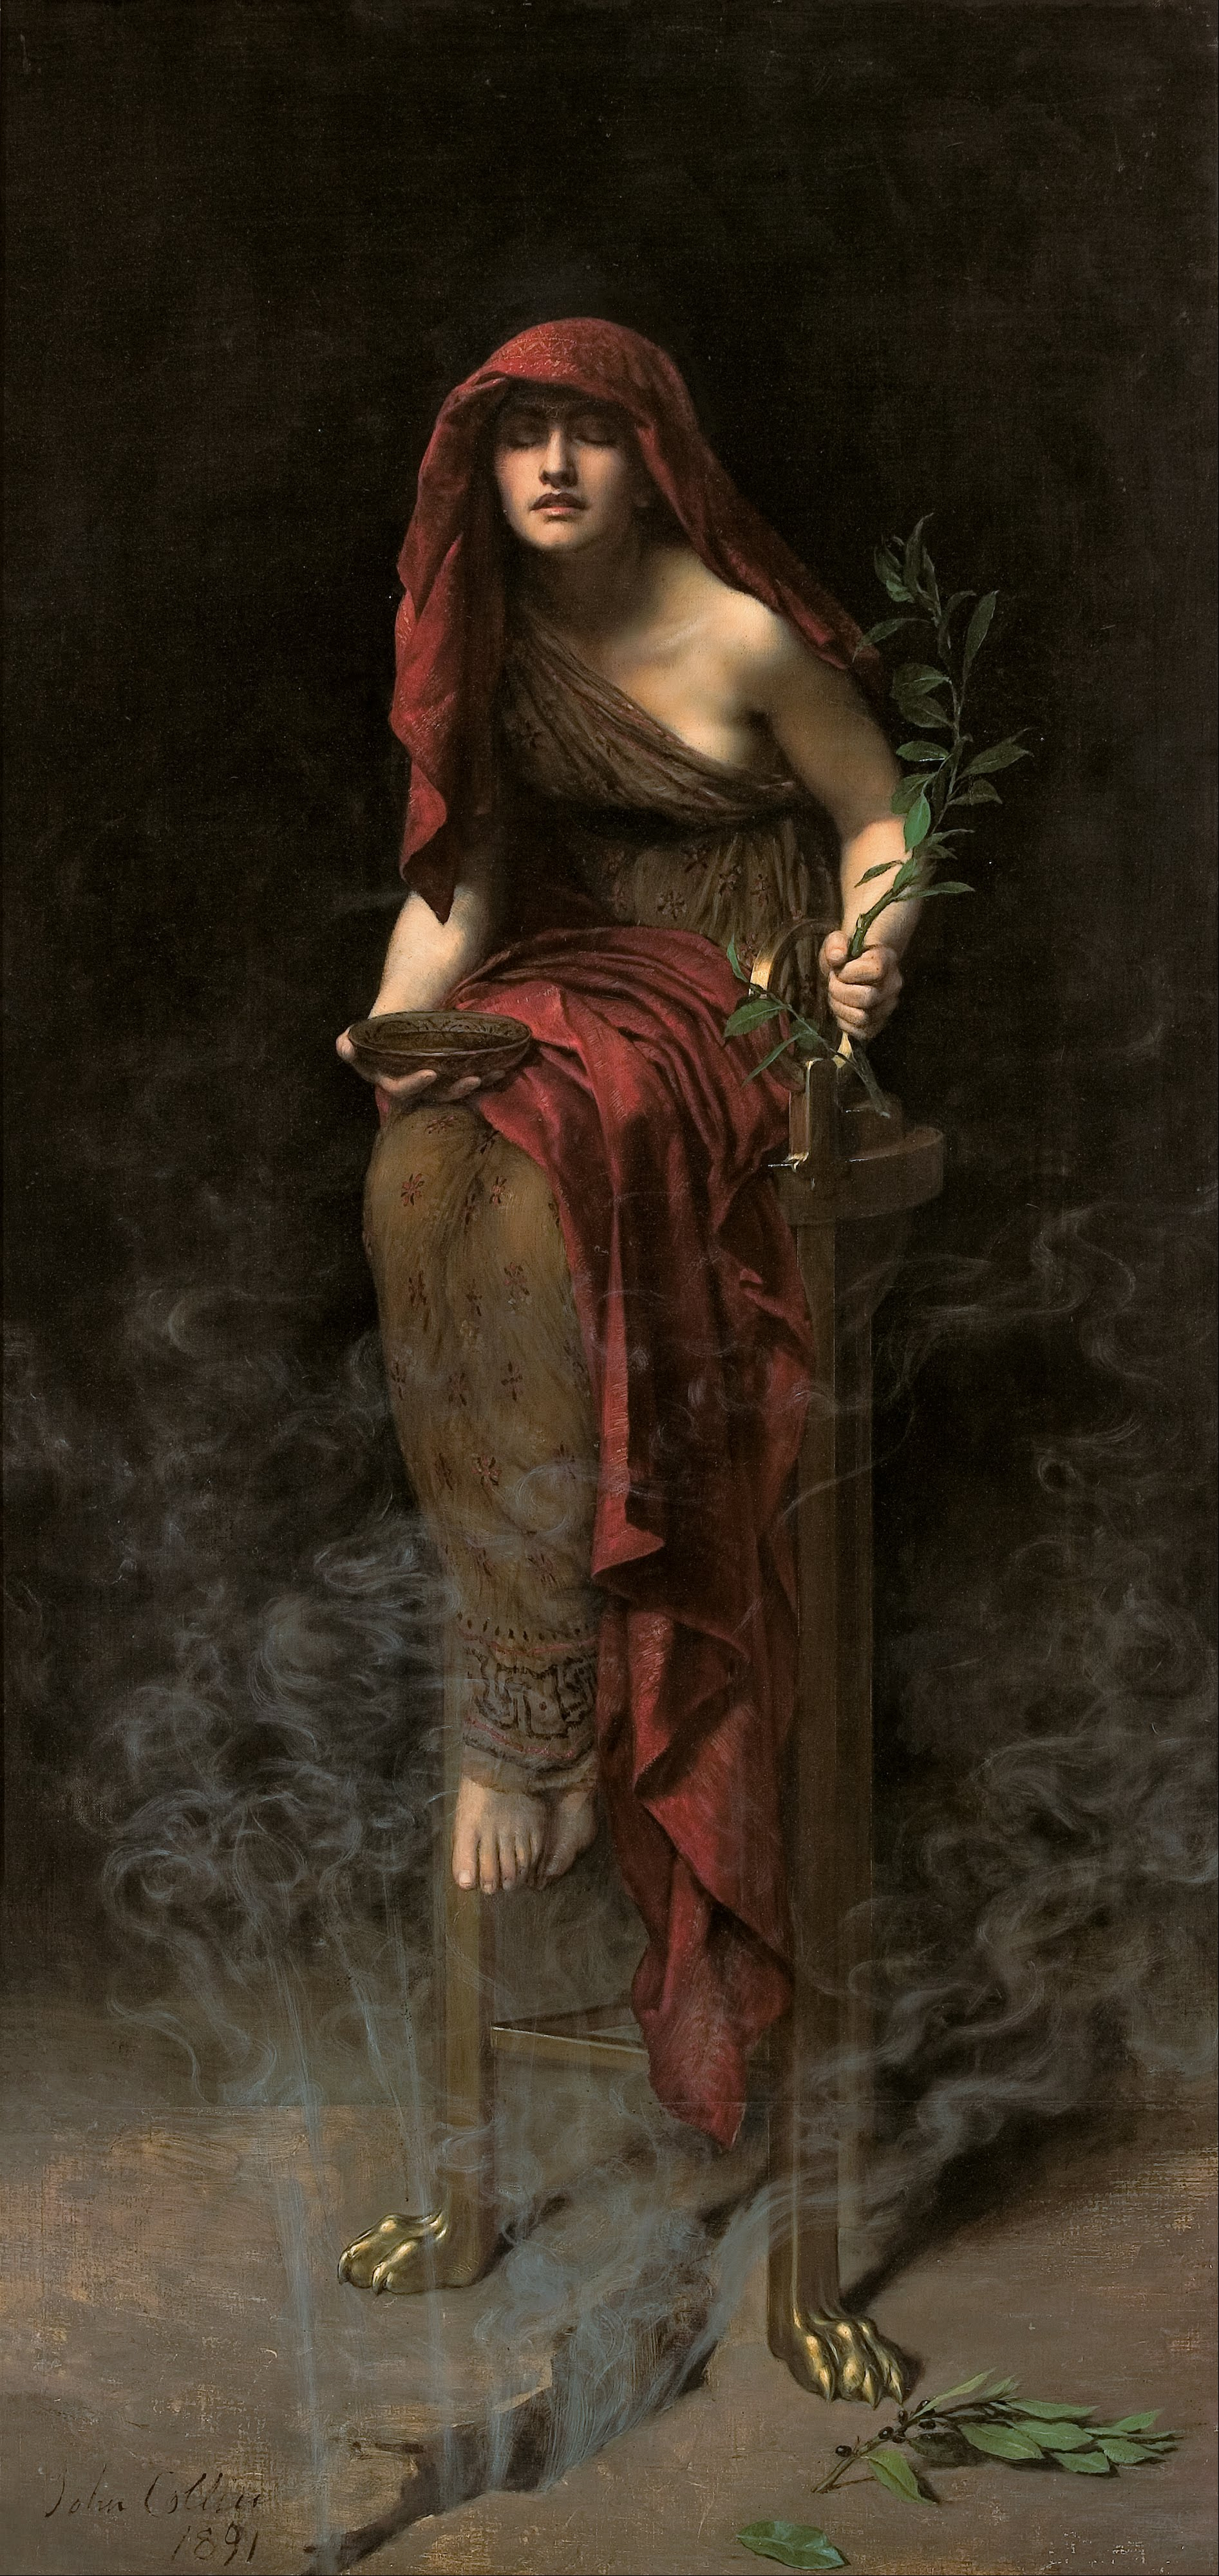
\includegraphics[width=0.3\textwidth]{pythia.jpg}
	\caption{Priestess of Delphi (1891) by John Collier.}
\end{figure}
\fi


\newpage
\section{Lattice based cryptography}
Gentry's work was a true breakthrough. It not only presented the first, fully homomorphic encryption scheme, but also gave researchers a very powerful tool, the \textit{bootstrapping}. From now on, all we need to construct another FHE scheme, is some suitable (one requirement would be to use a scheme based on ring rather than a group) SHE method, apply appropriate "squashing" to obtain the bootstrapping and we are done. In the following years this is exactly what happened in academia and the industry.

This section will mostly serve as a survey of the main developments towards more efficient fully homomorphic encryption using (ideal) lattices and their security based on computational hardness of the underlying problems. We adopt chronological narrative of the sections, starting with the oldest, the GGH algorithm, progressing through works on (ring-)LWE and eventually arriving at the work of Gentry \cite{gentry_phd} on ideal lattices and FHE. For a good survey on the lattice based cryptography, see for example \cite{two_faces}, \cite{book} chapter 6 or \cite{lattice-survey}.

\subsection{The GGH public key cryptosystem}
We will start this section with a somewhat simpler cryptosystem that was developed by Goldreich, Goldwasser and Halevi and presented in 1997 \cite{ggh}, called the GGH cryptosystem. This scheme, rather than using ideal lattices (i.e. lattices that are also ideals in the ring of integers), relies on general properties of lattices. Namely, the hardness of the SVP and CVP (see section \ref{hardness}).

\subsubsection*{Idea behind the scheme}
The basic GGH cryptosystem, as mentioned before, is based on the problem of finding the closest vector in the lattice $\mathcal{L}$ to a given point in the ambient space $\R^n$. We are given two bases, call them $\Bg$ and $\Bb$. The $\Bb$ will be our public key and $\Bg$ the secret key. The $\Bb$ consists of long and highly non-orthogonal vectors, as opposed to $\Bg$. Our secret message $\bm{m}$ is represented as a binary vector which we will use to form a linear combination $\bm{s} = \sum m_i \bm{v}_i^{bad} \in \mathcal{L}$ of the vectors in $\Bb$. We now add some small and random\footnote{some small note about the "randomness" of this e} error $\bm{e} \in \R^n$ to obtain the ciphertext $\bm{c} = \bm{s} + \bm{e} = \sum m_i \bm{v}_i^{bad} + \bm{e} \in \R^n$ - some point that is not in the lattice, but rather, very close to a point in it.\\
To decrypt, we can use our good basis $\Bg$ to represent $\bm{c}$ and, for example Babai's algorithm\footnote{Simply stated, if the vectors of the basis are sufficiently orthogonal to one another, then this algorithm solves \prob{approxCVP}. However, if the Hadamard ratio is too small, the algorithm fails to find the closest vector - \cite{book}.} to find $\bm{v}$ and represent it in terms of the basis $\Bg$ to recover $\bm{m}$. On the other hand, any eavesdropping adversary that is trying to learn our secret, is left with some bad basis that will be of no help in solving the CVP.

\subsubsection*{GGH construction - concretely}
\noindent\fbox{%
    \parbox{\textwidth}{%
$\alg{KeyGen}$:
\begin{itemize}
    \item Pick a basis $(\bm{v}_1, \bm{v}_2, \dots, \bm{v}_n) \subset \Z^n$ such that they are reasonably orthogonal to one another - i.e. with small Hadamard ratio. We will associatie the vectors $\bm{v}_1, \bm{v}_2, \dots, \bm{v}_n$ as the $n$-by-$n$ matrix $\bm{V}$ and let $\mathcal{L}$ be the lattice generated by these vectors. This is our good basis $\Bg$ - the \textbf{private key}.
    \item Pick an $n$-by-$n$ matrix $\bm{U}$ with integer coefficients and determinant $\pm 1$ and compute $\bm{W} = \bm{UV}$. The column vectors $\bm{w}_1, \bm{w}_2, \dots, \bm{w}_n$ of $\bm{W}$ are the bad basis $\Bb$ of $\mathcal{L}$ - the \textbf{public key}\footnote{As an alternative, in \cite{hnf}, Micciancio suggested to use the Hermite Normal Form (HNF) of $\Bg$ which essentially provides the worst possible lattice choice from both cryptoanalitical and efficiency point of view.}.
\end{itemize}
$\alg{Encrypt}$:
$\alg{Decrypt}$:
}} \\

The greatest drawback of GGH is that there were no proofs of security presented along the algorithm, only heuristic assumptions. This motivated researchers to look for possible exploits beased on the choice of parameters. Indeed, this scheme turned out to be insecure for most practical choices of the security parameter only 2 years later, in \cite{break1} and broken completely in \cite{break2}. Nonetheless, the ideas presented there have served as a basis for many schemes that are proven to be secure, like for example LWE, and has led to a plethora of applications.
\subsection{Learning With Errors}
Let us now begin with what went wrong in GGH. Namely, first prove the hardness of a problem, then use it to construct a secure and efficient cryptosystem. In this section we introduce \textit{Learning With Errors} (LWE) problem and the cryptosystem introduced by Oded Regev in \cite{regev} (he won the \href{https://eatcs.org/index.php/component/content/article/1-news/2670-2018-godel-prize}{2018 Gödel Prize} for this work). This very important work in the field of lattice based cryptography is, up to the date \krzys{im not sure if this statement is true, i need to look more into it}, one of the most efficient schemes with an actual proof of security. It has served as a foundation for countless subsequent works in the field.

\iffalse
\subsubsection*{Lattices - Part II}

\begin{definition}[Dual]
    For a lattice $\mathcal{L} \subset \R^n$ its $\Z$\textit{-dual} is
    $$ \mathcal{L}^{\vee} = \{ y \in \R^n : y \cdot \mathcal{L} \subset \Z \}.$$
    Here, the $\cdot$ means the usual dot product.
\end{definition}

We simply require that the elements of the dual are precisely those vectors that yield an integer when "multiplied" with an element of our lattice. Note that this is different from our standard definition of a dual. Namely, it is not the orthogonal compliment of our starting space, i.e. not all of the elements of the dual have 0 dot product against the vectors of the lattice.

\begin{example}
    Take $\mathcal{L}= \Z 
        \big(\begin{smallmatrix} 1\\2 \end{smallmatrix}\big) + 
        \Z \big(\begin{smallmatrix} 0\\ 1 \end{smallmatrix}\big)$
        To calculate the dual of $\mathcal{L}$ we need our $y = \big(\begin{smallmatrix}
          a\\b\end{smallmatrix}\big)$ elements to satisfy $a \in \Z$ and $2a + b \in \Z$ which is equivalent to asking $a \in (1/2)\Z$ and so $\mathcal{L}^{\vee} = \big(\begin{smallmatrix}
          1/2\\0
        \end{smallmatrix}\big)\Z + \big(\begin{smallmatrix}
          0\\1
        \end{smallmatrix}\big) \Z$
\end{example}

Note that $\mathcal{L}^{\vee}$ is itself a lattice of the same dimension.
\fi

\subsubsection*{LWE problem}
There are multiple equivalent definitions of this problem. We adopt the notation and approach introduced in the original paper by Regev. \\
The problem is parametrized by positive integers $n$, $m$\footnote{As it turns out, $m$ is of secondary importance here and is usually taken to be equal to $n$ itself.} and prime $q$, as well as an error distibution $\chi$ over $\Z_q$. It is now defined as follows. We are given $m$ equations of the form $(\bm{a}_i, b_i = \langle \bm{a}_i, \bm{s} \rangle + e_i)$ and are asked to find the vector $\bm{s} \in \Z_q^n$. Here, $\bm{a}_i$ are chosen uniformly and independently from $\Z_q^n$, $b_i \in \Z_q$ and $\langle \cdot, \cdot \rangle$ denotes the usual dot product. The errors $e_i$ are obtained by sampling independently from the probability distribution $\chi : \Z_q \rightarrow \R^{+}$ (\krzys{im not sure if he means the positive reals or something else}) on $\Z_q$. We will denote the problem of recovering $\bm{s}$ from such equations, by $\text{LWE}_{q, \chi}$ (learning with errors).

\begin{example}[From the introduction to \cite{survey_regev}]\label{lwe_ex}
    Given as input this set of equations, LWE asks us to find the vector $\bm{s} = (s_1, s_2, s_3, s_4) \in \Z_{17}^4$. In this case $n = 4$, $q=17$ and the error distribution is giving us $e_i = \{-1, 1\}$ with equal probability. 
\begin{align*}
    14s_1 + 15s_2 +5s_3 + 2s_4 & \approx 8 \, (\mod 17)\\
    13s_1 + 14s_2 + 14s_3 + 6s_4 & \approx 16\, (\mod 17) \\
    6s_1 + 10s_2 + 13s_3 + 1s_4 & \approx 3\, (\mod 17) \\
    10s_1 + 4s_2 + 12s_3 + 16s_4 & \approx 12\, (\mod 17) \\
    9s_1 + 5s_2 + 9s_3 +6s_4 & \approx 9\, (\mod 17) \\
    3s_1 + 6s_2 +4s_3 +5s_4 & \approx 16\, (\mod 17) \\
    \vdots & \\
    6s_1 + 7s_2 + 16s_3 + 2s_4 & \approx 3\, (\mod 17)
\end{align*}
In this case, $\bm{s} = (0, 13, 9, 11)$. Note that if not for the error, the secret would be very easy to find. Given about $n$ equations, we could recover $\bm{s}$ in an efficient way using Gaussian elimination. Inducing the error is what seems to render the problem untraceable for modern day algorithms.
\end{example}

The central part of \cite{regev} revolves around proving conjured hardness of LWE. Specifically, that for appropriately chosen $q$ and $\chi$, a \textit{quantum} reduction algorithm exists that approximates worst-case lattice problems. 
\begin{remark}
    At some point as well, we would like to find a \textit{classical} reduction algorithm that proves the hardness of the problem. This is because we understand classical computation in much more detail than its quantum equivalent. Using classical computers we have cracked Enigma and landed on the moon. In the meantime, only recently a factorization of the integer 15 was achieved on a quantum computer using Shor's algorithm - see \krzys{find source of that statement}. Returning to the reduction problem, Chris Peikert in his paper \cite{peikert_classical} from 2009 has done exactly this. However, it was done in a somewhat ``inefficient'' way. I.e. exponential many samples are needed in the classical reduction compared to polynomial amount in the quantum version. For more details see the paper by Peikert and compare it with the original approach from Regev. It remains still an open question \krzys{also not sure about that} if the reduction can be made efficiently fully classical.
\end{remark}
The result is loosely stated as follows.

\begin{theorem}[Theorem 1.1 in \cite{regev}]
    Let $n$, $q$ be positive integers and $\alpha \in (0, 1)$ be such that $\alpha q > 2 \sqrt{n}$. If there exists an efficient algorithm that solves $\text{LWE}_{q, \bar{\Psi}_{\alpha}}$, then there exists an efficient quantum algorithm that approximates the decision version of the shortest vector problem (\prob{GapSVP}) and the shortest independent vectors problem (\prob{SIVP}) to within $\tilde{O}(n/\alpha)$ in the worst case on any lattice of dimension $n$.	
\end{theorem}

Let us unwrap this statement. As said before, we need an appropriate choice of paramenters to obtain our results and $\alpha > 2\sqrt{n}/q$ is one of those choices (and requirements). It specifies the shape of the $\bar{\Psi}_{\alpha}$ distribution. This one is almost identical to the discrete Gaussian distribution over $\Z_q$ that is centered around 0 with standard deviation $\alpha q$\footnote{A comment from \cite{lattice-survey}: Originally, Regev considered the continuous Gaussian and rounded the result to the nearest integer. This does not exactly yield the discrete distribution but thanks to \cite{discr} we know how the problem can be fixed.}. The theorem can be rephrased as follows. Imagine that we have an efficient algorithm that solves the $\text{LWE}_{q, \bar{\Psi}_{\alpha}}$. Then, there exists a quantum solution to worst-case lattice problems, namely \prob{GapSVP} and \prob{SIVP}. Since we strongly believe that \prob{GapSVP} and \prob{SIVP} are difficult to solve (\cite{svp-hard}, \cite{reductions}, \cite{cvp-hard}) we are left with a difficult, yet efficient way to share secrets.

Oded Regev proceeds to prove this using various lemmas and results from few areas of mathematics like probability, lattice theory and quantum computing. We will now present an outline of the approach.\\
Recall that we want to prove, that being able to solve $\text{LWE}_{q, \chi}$ implies that we are able to solve standard worst-case lattice problems like \prob{GapSVP}.
\krzys{im not sure if i wanna include this at all} \\
\begin{remark}
    We are still faced with a problem that is inherent to all of modern-day cryptography. That is, we are assuming the hardness of the problem based on our inability to efficiently solve it. It might so happen that tomorrow someone finds an efficient (polynomial time) algorithm to find the shortest vector in a given lattice and our secrets are compromised. This is exactly what happened in the case of RSA cryptosystem when Shor found such efficient algorithm for integer factorization. There is not much we can do about it at least with our current approach to cryptography which is based on very precise complex-theoretic assumptions.
\end{remark}
\subsubsection*{LWE cryptosystem}
Now that we have a solid hardness assumptions, we can attempt to construct a cryptosystem that employs those results. The following public key cryptosystem was presented in the same paper. To keep the notation consistent with previous section, we will slightly deviate from the original.

We begin by specifying our parameters. Let us denote by $n$ our security parameter. As before, the scheme is characterized by two integers $m$ and $q$ and a probability distribution $\chi$ over $\Z_q$. To now make the scheme secure and correct, we should choose $q$ prime between $n^2$ and $2n^2$, $m = (1 + \epsilon)(n + 1) \log q$ for some arbitrary constant $\epsilon > 0$. We define the distribution $\chi$ to be $\bar{\Psi}_{\alpha (n)}$ where $\alpha (n) = o(1/(\sqrt{n} \log n))$ (recall from Section \ref{hardness} that it means $\lim_{n\to\infty} \alpha (n) \cdot \sqrt{n} \log n = 0$).\\

\begin{mdframed}
$\alg{KeyGen:}$
\begin{itemize}
    \item Choose $\bm{s} \in \Z^n_q$ uniformly at random. This is the \textbf{private key}.
    \item For $i = 1, \dots, m$ choose $m$ vectors $\bm{a}_i \in \Z^n_q$ independent from the uniform distribution. Additionally choose $m$ elements $e_i \in \Z_q$ independently according to $\chi$. The \textbf{public key} is the array of $m$ vectors of the form $(\bm{a}_i, b_i)$ where each $b_i$ is given by $b_i = \langle \bm{a}_i, \bm{s} \rangle + e_i$.
\end{itemize}
$\alg{Encrypt:}$\\
To encrypt a single bit we choose a random set $S$ uniformly among all $2^m$ subsets of $\{1, \dots, m\}$. The encryption is $(\sum_{i \in S} \bm{a}_i, \sum_{i \in S} b_i)$ if the bit is 0, and $(\sum_{i \in S} \bm{a}_i, \lfloor q/2 \rfloor + \sum_{i \in S} b_i)$ otherwise. \\
$\alg{Decrypt:}$\\
The decryption of a pair $(\bm{a}, b)$ is 0 if $b - \langle \bm{a}, \bm{s} \rangle$ is closer to 0 than to $\lfloor q/2 \rfloor$ modulo~$q$.
\end{mdframed}

\begin{example}
    Almost exactly like in the Example \ref{lwe_ex}, set $n = 4$, $q=17$, $m=4$ and $\chi = \bar{\Psi}_{1/2}$. We pick our \textbf{secret key} $\bm{s} = (2,1,3,7)$ and artificially (i.e. by design and not uniformly at random) pick
    \[ \bm{A} = (a_1, a_2, a_3, a_4) = 
	\begin{pmatrix}1 & 16 & 4 & 5\\
	    		16 & 4 & 5 & 1 \\
			4 & 5 & 1 & 16 \\
			5 & 1 & 16 & 4
	\end{pmatrix}. \]
	Take $e_1 = e_2 = 1$ and $e_3 = e_4 = -1$. Now we can compute the \textbf{public key} 
	\[ \bar{\bm{A}} = \begin{bmatrix} \bm{A} \\ \bm{b} \end{bmatrix} = 
	\begin{bmatrix} \bm{A} \\ \langle \bm{a}_i, \bm{s} \rangle + e_i \end{bmatrix}  = 
	\begin{pmatrix} 1 & 16 & 4 & 5 \\
	    16 & 4 & 5 & 1 \\
	    4 & 5 & 1 & 16 \\
	    5 & 1 & 16 & 4 \\
	    15 & 8 & 8 & 11
	\end{pmatrix}.
	\]
    To now encrypt a bit 1, we can take as our $S$ the set $\{1,2,4\}$ and output the encryption as
	    \begin{align*} \begin{pmatrix} 1 + 16 + 5 & (\lfloor 17/2 \rfloor =) 8 + 15\\
		16 + 4 + 1 & 8 + 8 \\
		4 + 5 + 16 & 8 + 8 \\
		5 + 1 + 4 & 8 + 11
		\end{pmatrix} & = \begin{pmatrix} 5 & 6 \\ 4 & 16 \\ 8 & 16 \\ 10 & 2 \end{pmatrix}
	    \end{align*}


\end{example}

\subsubsection*{Analysis}
Now, that we have finally defined a cryptographic scheme we need to verify it. The two remaining questions we now have are first, is this scheme correct? That is, does the decryption algorithm correctly evaluate back to the original message? This is much more difficult to prove compared to the scheme over the integers presented in \ref{int_she}. The following is a somewhat simpler version of Claim 5.2 in \cite{regev}.
\begin{claim}[Correctness]
    For the above choice of parameters and $e$ following the $\chi$ distribution we have
    \begin{equation} \Pr \Big[ |e| < \Bigl \lfloor \frac{q}{2} \Bigr \rfloor /2 \Big] > 1 - \delta(n) \end{equation}
    for some $\alg{negligible}$ function $\delta(n)$.
\end{claim}
This, in turn, implies that (this is Lemma 5.1)
\begin{theorem}
    The decryption is correct with probability $1 - \delta(n)$ where the $\delta(n)$ is some $\alg{negligible}$ function.
\end{theorem}

\begin{proof}
    Consider first the encryption of 0. It is given by $(\bm{a}, b)$ with $\bm{a} = \sum_{i \in S}\bm{a}_i$ and $b = \sum_{i \in S} b_i = \sum_{i \in S} \langle \bm{a}_i, \bm{s} \rangle + e_i$. Then the decryption gives us precisely $b - \langle \bm{a}, \bm{s} \rangle = \sum_{i \in S} e_i$. By our assumption, $\big| \sum_{i \in S} e_i \big| < \bigl \lfloor \frac{q}{2} \bigr \rfloor /2$ with probability at least $1 - \delta(n)$. In that case, it is closer to 0 than $\bigl \lfloor \frac{q}{2} \bigr \rfloor$ and thus correctly decrypts to 0. The case for the encryption of 1 is similar.
\end{proof}

Note that it seems almost trivial that we decrypt correctly, the scheme was designed in that way. This is only the case when we know the secret key $\bm{s}$ that is definitely not know to the public. This ties closely to the second and last question, that is, how secure the scheme is? We have established hardness based on average and worst-case lattice problems. However, it might be the case that our choice of parameters required for correctness, hinders on the security. This is resolved with the following theorem:
\begin{theorem}[Lemma 5.4 - Security]\label{pseudo-lwe}
    For any $\epsilon > 0$ and $m \geq (1 + \epsilon)(n + 1) \log q$, if there exists a polynomial time algorithm $\alg{W}$ that distinguishes between encryptions of 0 and 1 then there exists a distinguisher $\alg{Z}$ that distinguishes between $A_{\bm{s}, \chi}$ and $U$ for a non-negligible fraction of all possible $\bm{s}$.
\end{theorem}
\krzys{TODO: finish security}
"It turns out that when the modulus q is prime and polynomial in n, the search and decision variants are equivalent via an elementary reduction (but no such equivalence is known for larger q)." - quote from Peikert
For a thorough and less technical analysis than the one given in the original paper, the reader is encouraged to look into section 5.4 in \cite{Micci2009}.
\subsection{Ring-LWE}
One of the recurring problems in lattice-based cryptography is the key-size and general efficiency. In the GGH cryptosystem, the key-size is $\tilde{O}(n^4)$. In the system based on the hardness of LWE presented in the previous section, the size is in the range of $\tilde{O}(n^2)$\footnote{There are $m$ samples of length $n$. Turns out that for $m > n$, the problem can become only easier, but the same holds for $m \ll n$. Therefore, in most applications, $m$ is chosen to be roughly the size of $n$.}. As we will also see later, there is some minimal efficiency needed for the scheme in order to enable the boostrapping. Unfortunately, none of the schemes presented so far satisfy those criterions and so, we need to look for something better.

One idea to improve the inefficiency, is to assume some underlying structure of the space we are performing computations in. More precisely, assume that the $\bm{a}$ vectors from previous section are given to us in block of $n$ samples $\bm{a}_1, \bm{a}_2, \dots, \bm{a}_n \in \Z_q^n$ where all of the elements are related. Namely, $\bm{a}_1 = (a_1, \dots, a_n)$ is again chosen uniformly but each $\bm{a}_i = (a_i, \dots, a_n, -a_1, \dots, -a_{i - 1})$ is a ``skewed-rotation'' \krzys{there must be better word for this} of the initial $\bm{a}_1$. For example if $n = 4$ and $q = 17$ as before and $\bm{a}_1 = (1, 16, 4, 5)$ then $\bm{a}_3$ has the form $(4, 5, -1, -16) = (4, 5, 16, 1)$. Note that representing $n$ vectors now takes only $O(n)$ elements from $\Z_q$ rather than $O(n^2)$. The underlying structure is a ring, hence the name ring-LWE (or R-LWE), namely we replace the group $\Z_q^n$ by picking some ring $R$ of degree $n$ over $\Z$ and a positive modulus $q$ defining the quotient ring $R_q := R/qR$. In most of the cases (as well as in this exposition), $R$ is taken to be a \textit{cyclotomic} ring - i.e. $R_q = \Z_q[x]/\langle x^n + 1 \rangle$ for $n = 2^k$ which turns out to yield much simpler proofs for the desired results.

In the year 2010, V.Lyubashevski, C.Peikert and O.Regev presented their paper ``On Ideal Lattices and Learning With Errors Over Rings'' \cite{ring-lwe}. The main purpose of the paper was to ``translate'' the LWE problem onto a ring as was done with the SIS problem (by Micciancio \cite{ring-sis} but it is not presented in this paper) and followed the heuristic approach behind the NTRU\footnote{As mentioned by Peikert in his survey: ``The meaning of the acronym NTRU is somewhat mysterious; plausible candidates include "N th degree truncated polynomial ring" and "Number Theorists ’R’ Us."'' - \cite{lattice-survey}} cryptosystem \cite{ntru}. This in particular means first, defining the ring-LWE and later proving the hardness based on some difficult lattice problems like \prob{SVP} along with pseudorandomness of the ring-LWE distribution (analogous to \ref{pseudo-lwe} which we define later).

\subsubsection*{Definitions}





Chinese remainder theorem for rings --> Thm II.4.12 in Top's lecture notes. \\
For instance, they have unique factorization of ideals, and their fractional ideals form a multiplicative group; in general, neither property holds in $\Z[x]/\langle f (x) \rangle$ for monic irreducible $f (x)$, as demonstrated by the ring $\Z[x]/\langle x^2+3 \rangle = \Z[\sqrt{-3}]$. (For example, in this ring $4 = 22 = (1+\sqrt{-3})(1 - \sqrt{-3})$, but 2, $1 + \sqrt{-3}$, and $1 - \sqrt{-3}$ are all irreducible.)
Toward basing fully homomorphic encryption on worst-case hardness \\
One of the applications is \cite{qTESLA} signature scheme.

\subsection{Fully Homomorphic Encryption Using Ideal Lattices}
three ``generations'' of fhe schemes, first original gentry, smart and
explain here how we can construct a really nice homomorphic encryption scheme using ideal lattices \cite{gentry}. present the 
\subsubsection*{On Ideal Lattices and Learning With Errors Over Rings}
this is somewhat too difficult for me i think so ill just present main findings without proofs and details \cite{regev}, \\
First explain what lattices are. \\
How do lattices relate to LWE? The secret key is associated with a random vector. \\
then show how ring-lwe satisfies both of our requirements \cite{ring-lwe}, namely, the believed hardness for quantum computers (SVP or approximate SVP) and FHE. Show also the problem with ring-LWE because the lattices that are used there are ideal lattices which obviously possess more structure than "normal" lattices.


\newpage
\section{Homomorphic Encryption}
Fully Homomorphic Encryption (FHE) has been referred as the ``holy grail'' of modern cryptography as it was one of the most sought goals for the past couple of decades. First formally introduced by Rivest, Adleman and Dertouzos in \cite{primal} (at the time called ``privacy homomorphism''), shortly after the discovery of public key cryptography, it has been an open and elusive problem. Only ``recently'', in~2009, Craig Gentry proposed first FHE in his PhD thesis \cite{gentry_phd}. Since then, there has been a lot of development in the area like for example \krzys{TODO: finish developments of fhe}.

Simply stated, in homomorphic encryption we want our data to be secure but we also want to perform calculations on it. This is useful when we need a third party (e.g. someone with more computational power) to perform operations on our data while still retaining privacy. Alice can store her data somewhere on external server (for example the cloud) and ask to perform computations on it. We can for example query searches without the engine knowing what is actually being searched for.

In other words, we would like our encryption scheme -- call it $\E$ -- to satisfy the following. Say the ciphertexts $c_i$'s decrypt to messages $m_i$'s. Then we want
\[ \alg{Decrypt}_{\E}(c_1 + c_2) = m_1 + m_2, \qquad \alg{Decrypt}_{\E}(c_1*c_2) = m_1*m_2 \]
Equivalently, we want $\alg{Decrypt}$ to be a ring homomorphism. $\E$ being \textit{fully homomorphic} means that whenever $f$ is a composition of \textbf{arbitrily many} additions and multiplications, then $\alg{Decrypt}_{\E}(f(c_1, \dots, c_n)) = f(m_1, \dots, m_n)$\footnote{There are two more technical requitements, namely \textit{compactness of the ciphertexts} and \textit{efficiency} but we will not consider them in this paper.} which is also refered to as the \textit{correctness} of the scheme.

\begin{remark} \label{algs}
    Typically, an encryption scheme $\mathcal{E}$ is a tuple of $\alg{KeyGen}_{\E}$, $\alg{Encrypt}_{\E}$ and $\alg{Decrypt}_{\E}$ (representing the key-generation, encryption and decryption respectively), all of which we require to be \textit{efficient} -- i.e. run in time poly($\lambda$) - polynomial in the security parameter $\lambda$ that represents the bit-length of the keys (see for example \cite{katz} or \cite{book} for more details on the abstract build of a encryption scheme). A homomorphic encryption scheme has a fourth algorithm -- $\alg{Evaluate}_{\E}$ which we associate with some set of \textit{permitted functions}. In our case this will simply be $\alg{Add}_{\E}$ and $\alg{Mult}_{\E}$ which we will introduce in further sections. Adopting the notation from \cite{easy_fhe} we will denote by $\mathcal{F}_{\E}$, the generalized set of such functions.
\end{remark}

One might ask a question now, how secure can such scheme ultimately be? After all, we are giving the adversary a quite powerful tool in the form of being able to compute (ultimately) \textit{any} function on our data.

\subsection{Somewhat Homomorphic Encryption}\label{int_she}
Before we introduce the solution on to how to construct such FHE presented by Gentry, we will start with something slightly simpler, introduced in \cite{int_scheme} by van Dijk et al. Their scheme works over the integers rather than lattices but relies on a similar assumption. Namely, that finding the greatest common divisor of many ``noisy'' multiples of a number is computationally difficult. We will come back to this problem later. To keep the exposition compact, we will avoid specifying most parameter choices.

\subsubsection*{Symmetric Key Scheme}
We begin with the symmetric key scheme. We take our message to be a bit $m \in \{0,1\}$. The private key is an odd integer $p$ (no necessarily prime). To encrypt our message $m$, we choose integers $q$ and $r$ at random (such that the magnitude of $2r$ is smaller than $p/2$). We obtain the ciphertext $c$ by computing: 
\begin{equation}c = pq + 2r + m.\end{equation}
If we now want to decrypt our message, simply compute $(c \mod p) \mod 2$. \\
Let's say we have two messages $c_1$ and $c_2$. Then we can compute:
$$ c_1 + c_2 = m_1 + m_2 + 2(r_1 + r_2) + p(q_1 + q_2),$$
$$ c_1 * c_2 = m_1 * m_2 + 2(m_1r_2 + m_2r_1 + 2r_1r_2) + p(m_1q_2 + m_2q_1 + 2(r_1q_2 + r_2q_1) + pq_1q_2)$$
where we can see that the noise grows with each operation and the message becomes impossible to decrypt after we do too many of them. If we can assure that $2(m_1r_2 + m_2r_1 + 2r_1r_2)$ is small enough - i.e. smaller than $p$\footnote{When $2r > p$ then it might be the case that $2r = 1 \mod p$ and so $pq + 2r + m \mod p = 1 + m \neq m$.} - then we can assure that $\alg{Decrypt}(c_1 * c_2)$ evaluates correctly to the starting $m_1 * m_2$. Notice that $\alg{Decrypt}$ removes all the noise. This will be useful later for ``bootstrapping'' - a term introduced later on.

This simple encryption scheme is thus somewhat homomorphic as per definition by Gentry in \cite{gentry_phd} – namely, it can be used to evaluate low-degree polynomials over encrypted data. Further on in the Section 6 of \cite{int_scheme}, van Dijk et al. use the techniques (called bootstrapping and squashing) to lift it to a Fully Homomorphic Scheme.
\subsubsection*{Public Key Scheme}
The public key scheme is build very similarly. The private key $p$ stays the same. For the public key, sample $x_i = p q_i + 2r_i$ for $i = 0, 1, \dots, t$ where the $q_i$ and $r_i$ stay as before. The $x_i$ may be viewed as encryption of 0 under the symmetric key scheme. The $x_i$ are now taken s.t. $x_0$ is the largest, odd and $x_0 \mod p$ is even.

To now encrypt a message $m \in \{0,1\}$, chose a random subset $S \subseteq \{1, 2, \dots, t\}$ and a random integer $r$, and output
\begin{equation} c = (m + 2r + 2\sum_{i \in S} x_i) \mod x_0.\end{equation}
To decrypt, we again output $m = (c \mod p) \mod 2$.

The security of this preliminary SH scheme relies on the \textit{Approximate GCD Problem}\footnote{Later in \cite{revisited}, a reduction was constructed to LWE. This means, that under few more assumptions, this problem (and by extension any scheme based on it) is as secure as one based on LWE.}. In the simplest case, Euclid has shown us, that given two integers $c_1$ and $c_2$, it is easy to compute their $\gcd$. However, suppose now that $c_1 = p \cdot q_1 + r_1$ and $c_2 = p \cdot q_2 + r_2$ are ``near'' multiples of $p$, where $r_1$ and $r_2$ is some small noise sampled at random. This turns out to be much more difficult. In fact, if we pick our values appropriately (see \cite{easy_fhe} Section 3.4 and \cite{int_scheme} Section 3 for details) we do not know any efficient (running in polynomial time) algorithm even if we are given arbitrarily many samples $c_i = r_i + p \cdot q_i$.

However, this comfortable security comes at great cost because, as shown in \cite{int_scheme}, the parameters chosen to assure the secrecy, yield a scheme that has complexity of $\tilde{O}(\lambda^{10})$ where $\lambda$ is our security parameter (the greater it is the more secure message). As a small example, consider $\lambda = 10$ as the (small) key size. To now encrypt a single(!) bit, it will take approximately $10^{10}$ operations. On a modern laptop this would take a little less than 5 seconds. To send the message `hello', we need to use 5 letters $\cdot$ 16-bits per letter $= 5\cdot 16\cdot5 = 650$ seconds which is almost 11 minutes! As one can imagine, this is completely impractical for most applications.

\subsection{Fully Homomorphic Encryption}
We will now present the main idea introduced in Gentry's PhD thesis \cite{gentry_phd}. Namely, what is bootstrapping, why do we need it and how does it work. % how can we make use of ideal lattices to create a encryption scheme that can handle an arbitrary amount of functions. We will proceed in parallel with the original by introducing the idea of ``bootstrapping'', through a construction of a suitable SH scheme (this is where the ideal lattices show up) and finishing with the ``squashing''.

\subsubsection{Boostrapping}
We are faced with a problem. Because our method relies on some error being added to the message, it builds up after we perform operations on our data. The scheme $\E$ can handle functions in a limited set $\mathcal{F}_{\E}$ until the noise becomes too large. Is there a way for us to somehow expand this set and yet retain the homomorphic properties of the scheme? Can we, further on, expand this set to include an arbitrary polynomial function? The answer turns out to be yes. As shown by Gentry, one of the requirements for this is that the scheme can decrypt its encryption correctly ``and some''. A bit more formally, we require that the $\alg{Decrypt}_{\E} \in \mathcal{F}_{\E}$. This part will be a brief explanation of what the bootstrapping is and how we can achieve it using (also introduced in the same paper) ``squashing''.

\begin{remark}
  In cryptography, which is a field in the intersection of mathematics and computing science, instead of general functions, one often considers a \textit{circuit} instead. Roughly speaking, a circut is a translation of what a mathematician thinks when they say ``function''. It consists of (finite amount) of gates which are just boolean functions. For example there is a $\alg{NOT}$ gate that takes a bit $b \in \{0,1\}$ and outputs $b + 1$, where all the operations are performed modulo 2. Others include for example $\alg{XOR}$ - this is an exclusive logical $\alg{OR}$ - or $\alg{NAND}$ which is a $\alg{AND}$ followed up by a $\alg{NOT}$ gate. From a theoretical point of view, one can use solely a $\alg{NAND}$ gate to represent any circuit and thus we will be mostly concerned with that one.
\end{remark}

Imagine we have a SH scheme $\E$ (one can think of the one from previous section as a concrete example) that is correct for its own decryption circuit augumented by an $\alg{NAND}$ gate. We call such scheme \textit{bootstrappable}. As shown in the paper, one can use this circuit to create a (leveled) fully homomorphic encryption $\E^{(d)}$. It is called \textit{leveled} because the correctnes depends on the ``depth'' (or the level) $d$ of the circuit making it depend on $d$. It can be show that by appropriately augumenting the public key, such leveled scheme can be made independent of depth and thus made into a \textit{fully homomorphic} one. Moreover, if the scheme itself is secure\footnote{The precise security mentioned is the semantic security against chosen plaintext attacks. One can think of it as requiring that the same message $m$ has different outputs $c$ on different runs of the same encryption algorithm (it is non-deterministic). See \cite{katz} or \cite{lattice-survey} for a more precise definition.}, then so is any $\alg{Evaluate}_{\E^(d)}$ algorithm. All of this is captured in the following theorem.

\begin{theorem}[\cite{gentry}]\label{boot}
  One can construct a (semantically secure) family $\{ \E^{(d)} \}$ of leveled fully homomorphic encryption schemes from any (semantically secure) bootstrappable encryption scheme $\E$.
\end{theorem}

Why is this the correct requirement for a FHE? Suppose that there is an ``error'' associated with each ciphertext, just like in the scheme from Section \ref{int_she}. Then, as also noted there, after we perform one operations too many, the error builds up soo much that we are no longer able to decrypt correctly. We would therefore like to somehow make the error small enough again and ``refresh'' the ciphertext without using the secret key. Clearly we could get rid of the error completely if we were to decrypt it and create a ``fresh'' ciphertext of the same message. This is the precisely the idea, to decrypt the message but do it homomorphically! We obtain a homomorphic encryption by encrypting homomorphically -- we are bootstrapping. Gentry's idea on how to do it, was by appending the encryption of the secret key in the public key itself.

\begin{remark}
Note that this requires another assumption called ``circular security'' or KDM (Key Dependent Message) security. That is, we are assuming that the publication of the encryption of a secret key does not leak any valuable information about the key itself. This is however very difficult to prove in practice but also no known attacks are know and hence it is just assumed along.
\end{remark}

One last question we have is, why do we even need the error? Cannot we create a \textit{semantically} secure encryption scheme that does not depend on any ``error'' to hide the message, and consequently, create a FHE without any sort of bootstrapping? It turns out that it is in fact not possible. Before we present the reason for this, let us motivate why we care about the semantic security so much in the case of HE.

\begin{example}
	Using cloud computing as an example, imagine that after we stored few files in the cloud, we want to retrive files from the cloud that contain the \textit{Answer to the Ultimate Question of Life, the Universe, and Everything}. We thus homomorphically query the engine for the file number 42. But can't the cloud just ``notice'' that the encryption of the file it is sending us now is the same as the encryption of the \textit{Answer to the Ultimate Question of Life, the Universe, and Everything}? It cannot, if our encryption is semantically secure, because in that case, it is difficult to tell if two ciphertexts encrypt the same message.
\end{example}

Let us now get back to why we need the error. For any \textit{deterministic} algorithm (like \alg{AES} or \alg{RSA}) that encrypts $m$ as $c$ every time it is run, any adversary can check if any $m_0$ encrypts as $c$ and compare the two. Thus, by definition, such scheme cannot be semantically secure. We thus need a \textit{probabilistic} algorithm that gives us different output every time it is run. This implies some sort of randomizing the ciphertext which can only be done (to our understanding) using some error to mask the message. Therefore we need some sort of ``bootstrapping'' (which is not necessarily the one mentioned above, this is only one way to achieve FHE but there could be more) to create a FHE.

\paragraph{How to bootstrap}
We will not present the precise idea behind \textit{bootstrapping}. To this end, recall that our generic homomorphic scheme $\E$ consists of four algorithms. These are:
\begin{enumerate}
	\item $\alg{KeyGen}_{\E}$ which generates the public and secret keys -- pk and sk respectively.
	\item $\alg{Encrypt}_{\E}(\text{pk}, m)$ which encrypts the message $m$ from the plaintext space $\mathcal{P}$ under the public key $\text{pk}$ and outputs the ciphertext $c$.
	\item $\alg{Decrypt}_{\E}(\text{sk}, c)$ which decrypts the ciphertext $c$ using the secret key $\text{sk}$.
	\item $\alg{Evaluate}_{\E}(\text{pk}, f, c_1, \ldots, c_t)$ which evaluates the function $f \in \mathcal{F}_{\E}$ from the set of permitted functions on the ciphertexts $c_1, \ldots, c_t$ using the public key pk.
\end{enumerate}
We shall now construct a new algorithm which we will call $\alg{Recrypt}_{\E}$ using only those four above. For simplicity, we assume that our plaintext space is just $\{0,1\}$. Imagine we have a valid ciphertext $c_1$ that encrypts $m_1$ under the public key pk$_1$. In order to decrypt it homomorphically, assume additionally that we have the secret key sk$_1$ encrypted under another public key pk$_2$ -- denote this encryption by $\hat{\text{sk}}_1$ (\krzys{idk how to make it span the whole variable}). Define now the following algorithm:\\
$\alg{Recrypt}_{\E}(\text{pk}_2, \alg{Decrypt}_{\E}, \bar{\text{sk}}_1, c_1)$:


\begin{align*}
	\text{Set } \hat{c}_1 & \leftarrow \alg{Encrypt}_{\E} (\text{pk}_2, c_1) \\
	\text{Set } c_2 & \leftarrow \alg{Evaluate}_{\E} (\text{pk}_2, \alg{Decrypt}_{\E}, \hat{\text{sk}}_1, \hat{c}_1) \\
	\text{Return } c_2 &
\end{align*}

Here we use the encryption of our secret key to evaluate the decryption function homomorphically under a new public key. Now we can see why we need the assumption that the scheme is KDM secure. Since the encryption of sk$_1$ is public, we need to make sure it does not leak any information about it. The statement of the Theorem \ref{boot} should now be intuitively clear. As long as the scheme $\E$ can evaluate its own decryption function, and the $\alg{Recrypt}$ algorithm leaves the new message with less error than we began with, we can use $\E$ to construct a leveled FHE scheme. In order to now evaluate \textit{any} function on our data, we would also like our scheme to correctly evaluate a $\alg{NAND}$ gate (recall that we can create any gate using a finite combination of $\alg{NAND}$ gates) in order to make some progress before the error ``blows up''.

\subsubsection{Simple lattice based scheme}
The motivation for the choice of lattices as opposed to number theoretic constructions (like RSA or ElGamma for example, which are based on exponentiation), is that the former has few desirable properties. Firstly, the lattices have lower decryption complexity and are therefore more suitable as a bootstrappable encryption scheme. Next, one requires not only one supported homomorphism like addition but also the multiplication -- lattices as ideals poses both. Those factors among many others, (see \cite{gentry} for more details) have led to the choice of \textit{ideal lattices}.

The idea behind the encryption is somewhat similar to the one of GGH. That is, we are going to fix a basis for a lattice (which is an ideal), publish the bad basis as the public key and keep the good basis as a secret key. The security of this scheme is based on the Ideal Coset Problem\footnote{Later, in 2010, Gentry showed that the scheme can be based on the worst-case \prob{BDD} problem -- \cite{worst-case}.} (\prob{ICP}) introduced below. Briefly stated, given an element of some ring $t \in R$, the \prob{ICP} asks us to distinguish between a representative of a coset taken from some distribution over an arbitrary ring and a uniform sample.

For a ring $R$ and a basis\footnote{By the word ``basis'' we simply mean the set of generators for the ideal but we use that instead to highlight the connection between the ideals and lattices as well as keep it consistent with Gentry's work.} $\B_{\I}$ for an ideal $\I \subset R$, we use the notation $R \mod \B_{\I}$ to represent the set of $r + \I$ for $r \in R$.

\begin{definition}[Ideal Coset Problem]
	Fix a ring $R$ along with an ideal $\I \subseteq R$ and sample an element $r \in R$ given a sampling algorithm \alg{Samp}. Now pick a basis $\B_{\I}$ for the ideal $\I$. Given the basis $\B_{\I}$, the challenger is asked to distinguish between $t \equiv r \mod \B_{\I}$ and $t$ being chosen uniformly.
\end{definition}
Few remarks are in place now. Firstly, this definition hides few details in favour of clearer notation. As one, we actually fix some ideal $\J \subseteq R$ such that $\I$ and $\J$ are coprime (i.e. $\I + \J = R$) first, and then, with respect to such $\J$, we instantiate the $\I$. This will become evident later in this section why this is required. Secondly, the procedure somewhat depends on the efficiency of those choices. One example would be how to pick such coprime ideals as well as how to sample the $r$ from the ring itself. The questions (partially) are answered in the paper \cite{gentry_phd} itself.

From now on, let $R$ be an arbitrary ring, and set $\I, \J \subset R$ as two coprime ideals of $R$.  We will also be using a sampling algorithm which we call \alg{Samp}$(x, \B_{\I} , R, \B_{\J})$ that samples from the coset $x + \I$. Let us now introduce the scheme in terms of rings and ideals only.

\begin{mdframed}
	$\alg{KeyGen}(\B_{\I}, R$) \\
	Generate two basis for $\J$, $\B_{\J}^{sk}$ and $\B_{\J}^{pk}$. The \textbf{public key} $pk$ includes $R$, $\B_{\I}$, $\B_{\J}^{pk}$ and the sampling algorithm \alg{Samp}. The \textbf{secret key} $sk$  also includes the $\B_{\J}^{sk}$. We denote by $\mathcal{P}$ the plaintext space which is (a subset of) $R \mod \B_{\I}$.\\
	$\alg{Encrypt}(\text{pk}, m)$ \\
	For a message $m \in \mathcal{P}$, set $c' \leftarrow$ \alg{Samp}$(m, \B_{\I}, R, \B_{\J}^{pk})$ and output $c \equiv c' \mod \B_{\J}^{pk}$.\\
	$\alg{Decrypt}(\text{sk}, c)$ \\
	For the ciphertext $c$, output $(c \mod \B_{\J}^{sk}) \mod \B_{\I}$.\\
	$\alg{Evaluate}(\text{pk}, f, C)$ \\
	This algorithm takes a set of ciphertexts $C = (c_1, \ldots, c_t)$ and applies the function $f \in \mathcal{F}_{\E}$ using the public key pk. It outputs $f(c_1, \ldots, c_t)$. Since we only support two operations from the ring, $f: R \rightarrow R$ needs to be a homomorphism.
\end{mdframed}

Having the bootstrapping in mind, we should pay close attention to the correctness of the decryption algorithm. Before proving it, let us state few definitions first.

\begin{definition}
	Let $X_{Enc}$ be the image of $\alg{Samp}$. Notice that all ciphertexts output by $\alg{Encrypt}$ are in $X_{Enc} + J$. Let $X_{Dec}$ equal $R \mod \B^{sk}_{\J}$, the distinguished representatives of cosets of $\J$ wrt the secret basis $\B^{sk}_{\J}$.
\end{definition}

\begin{definition}[Permitted Functions]
	Let
	\[ \mathcal{F}_{\E} := \{ f : \forall (x_1, \ldots, x_t) \in X_{Enc}^T, f(x_1, \ldots, x_t) \in X_{Dec}. \} \]
	In other words, $\mathcal{F}_{\E}$ is the set of those functions of which output will always be in $X_{Dec}$ when the input is from $X_{End}$.
\end{definition}
Aditionally, we say the $\hat{c}$ a \textit{valid ciphertext} if it equals $\alg{Evaluate}$(pk, $f, (c_1, \ldots, c_t)$ for some function $f \in \mathcal{F}_{\E}$. We can now state and prove the correctness of our scheme.
\begin{theorem}[Correctness]
	Assume $\mathcal{F}_{\E}$ is a set of permitted functions containing the identity. $\E$ is correct for $\mathcal{F}_{\E}$ –- i.e., $\alg{Decrypt}$ correctly decrypts valid ciphertexts.
\end{theorem}
\begin{proof}
	For $C = \{c_1, \ldots, c_t\}, c_k = m_k +i_k +j_k$, where $m_k \in \mathcal{P}, i_k \in \I, j_k \in \J$ and $m_k +i_k \in X_{Enc}$, we have
	\begin{align*}
		\alg{Evaluate}(\text{pk}, f, C) = & f(C) \mod \B_{\J}^{\text{pk}} \\
		= & f(m_1 +i_1 +j_1, \ldots, m_t+i_t+j_t) \mod \B_{\J}^{\text{pk}} \\	
		\in & f(m_1 +i_1, \ldots, m_t +i_t) + \J.
	\end{align*}
	If $f \in \mathcal{F}_{\E}$, then we have $f(X_{Enc}, \ldots, X_{Enc}) \in X_{Dec}$ and so
	\begin{align*}
		\alg{Decrypt} & (\text{sk}, \alg{Evaluate}(\text{pk}, C)) \\
		& = f(m_1+i_1, \ldots, m_t +i_t) \mod \B_{\I} \\
		& = f(m_1, \ldots, m_t)
	\end{align*}
	as required.
\end{proof}

Once we have the correctness, we can focus on the actual implementations of any fully homomorphic schemes. This in turn implies that we should pay very close attention to the size of $X_{Enc}$ and $X_{Dec}$. Namely, we want to maximize $X_{Dec}$ and minimize $X_{Enc}$ (while still retaining security). This is where we introduce the lattices.

\subsection{Further developments in FHE}
Since the inception of FHE, many new ideas have emerged as potential replacement for the details in the implementation in Gentry's work. In this section, we will briefly introduce some of such techniques and ideas. Finally the work we have done on LWE and its ring equivalent will pay off as we can rely on those results to abstractly create FHE scheme \krzys{i dont like this sentence but idk how to make it prettier}. 

\subsubsection{FHE from the standard LWE}
 One of such ideas is to replace the ideal lattices by an LWE sample instead. Let us now attempt to construct a SH scheme that is using the LWE assumption along the ideas presented in \cite{fhe-lwe}. Recall that a LWE$_{q, \chi}$ is specified by the odd modulus $q > 2$ and error distribution $\chi$. It provides us with the LWE distribution that we called $A_{s, \chi}$ where $\bm{s}$ was a random vector representing the secret key outputting us samples of the form
\[A_{s, \chi} \rightarrow (\bm{a}, b) = (\bm{a}, \langle \bm{a}, \bm{s} \rangle + e),\]
where $e$ was drawn from some distribution $\chi$ (usually taken to be the discrete Gaussian distribution with small standard deviation) over $\Z_q$ for $q$ prime\footnote{Since we will be using the decision version of the problem, we need to assume $q$ to be prime.}. We can now imagine a scheme that works as follows: to encrypt a single bit $m \in \{0,1\}$ using a secret key $\bm{s}$, draw a sample from $A_{s, \chi}$ and output the ciphertext
\[ c \; = \; (\bm{a}, b = \langle \bm{a}, \bm{s} \rangle +2e +m) \; \; \; \in \Z_q^n \cross \Z_q \]
Note that we have replaced the error $e$ with its two-times multiple in contrast to the original formulation by Regev as can be seen in Table \ref{lwe-enc}. This is not a problem at all because 2 and $q$ are coprime. To decrypt the message, first compute $\langle \bm{a},\bm{s} \rangle$ and substract that from $b$, giving $2e + m \mod q$ which, since $e \ll q$, is actually equal to $2e +m$ exactly. Finally, reduce modulo 2 and we are left with the original message $m$.

The scheme is clearly additively homomorphic. The issue arises when we try to multiply two ciphertexts. As shown in \cite{one-mult}, the (slight variation of) this scheme supports only a \textit{single} homomorphic multiplication with the expense of huge blowup in the ciphertext size.

To see how this is the case, consider a symbolic function $f_{\bm{a},b} : \Z_q^n \rightarrow \Z_q$ defined as:
\[f_{\bm{a}, b}(\bm{x}) = b - \langle \bm{a, x} \rangle \mod q = b - \bm{a}_i \bm{x}^i \; \; \; \in \Z_q \]
where we are using Eisenstein notation to represent elements $\bm{x} \in \Z_q^n$ (the transpose of the first element is implicit). Note now that the decryption is nothing else but evaluating this function on the secret key $\bm{s}$ and taking the result modulo 2. We can now define addition and multiplication using this function. Addition is straightforward, $f_{\bm{a}, b}$ is a linear function and so sum of two linear functions is still linear. Symbolically, $f_{\bm{a},b}(\bm{x}) + f_{\bm{a}',b'}(\bm{x}) = f_{(\bm{a}+\bm{a}',b+b')}(\bm{x})$ will represent the homomorphically added ciphertext $(\bm{a}+\bm{a}',b+b')$. Similarly, multiplying two such functions gives us:\krzys{i think ill get rid of eisenstein notation coz im not really consistent with it}
\begin{equation}\label{mult}
  \begin{split}
  f_{\bm{a},b}(\bm{x}) \cdot f_{\bm{a}',b'}(\bm{x}) & = ( b - \bm{a}_i \bm{x}^i) \cdot ( b' - \bm{a}'_i \bm{x}^i ) \\
						    & = h_0 + h_i \cdot \bm{x}^i + h_{i,j} \cdot \bm{x}^i \bm{x}^j,
\end{split}
\end{equation}
which yields us a second degree polynomial with coefficients $h_{i,j}$ that can be computed by expanding the parenthesis of the upper equation. The decryption is as before, that is evaluating at $\bm{s}$ and reducing modulo 2. Hence, the scheme is trully homomorphic. Unfortunately, nothing in life comes for free and indeed, the multiplication which took a ciphertexts of size $n+1$, expanded it to the one of size approximately $n^2/2$. As one might imagine this is completely unacceptable from an efficiency point of view and surely not enough for bootstrapping. This is where the main contribution of \cite{fhe-lwe} comes in -- the \textit{re-linearization} technique.
\paragraph{Re-linearization}
The goal is to reduce the ciphertext blow-up for multiplication. As turns out we can actually reduce the result back to just a $n+1$ size assuming something that resembles KDM security or ``circular security'' - i.e. we need to assume that the encryption of a secret key does not leak any information about it. However, the key difference is that we encrypt all of the linear and quadratic terms of $\bm{s}$ but using a different key, call it $\bm{t}$. More precisely, we encrypt numbers $\bm{s}^i$ as well as $\bm{s}^{i,j}$ using the new secret key $\bm{t}$. The adjusted equation \ref{mult} with $\bm{s}$ plugged in for $\bm{x}$ now (approximately) looks like: 
\begin{align*}
  %b^i = \langle \bm{a}^i, \bm{t} \rangle + 2e^i +\bm{s}^i \approx \langle \bm{a}^i, \bm{t} \rangle + \bm{s}^i \\
  %b^{i,j} = \langle \bm{a}^{i,j}, \bm{t} \rangle + 2e^{i,j} +\bm{s}^{i,j} \approx \langle \bm{a}^{i,j}, \bm{t} \rangle + \bm{s}^{i,j} \\
  & h_0 + h_i \cdot \bm{s}^i + h_{i,j} \cdot \bm{s}^i \bm{s}^j\\
  = \; \; & h_0 + h_i \cdot (b^i - \langle \bm{a}^i, \bm{t} \rangle) + h_{i,j} \cdot (b^{i,j} - \langle \bm{a}^{i,j}, \bm{t} \rangle), 
\end{align*}
which is just a linear function in $\bm{t}$! The key take-away is that multiplying the two linear functions and later re-linearizing, gives us another linear function that, when evaluated in $\bm{t}$, outputs the product of the original messages.

\subsubsection{FHE from the ring-LWE}
A step forward in losing the need for KDM security (or circular security) was presented by Z. Brakerski and V. Vaikuntanathan in \cite{fhe_rlwe}. There, they have used the ring-LWE assumptions to create a FHE scheme with provable security for KDM. The scheme is relatively simple thanks to the assumptions that guarantee security based on ring-LWE assumptions. We will begin the construction with the SH scheme and later prove the circular security.

\subsubsection*{Ring-LWE SHE scheme}
The assumptions for this scheme are almost identical as for the ring-LWE, i.e. we take $a$ randomly from some ring that we call $R_q$ and the error term $e$ from some distribution $\chi$ (again, usually taken to be Gaussian). Since we will be basing our scheme on the decision version, we should take $q$ to be prime just like in the previous scheme. For compactness we avoid a precise formulation of the parameters, we refer the reader to the Section \ref{ring-lwe} on the hardness of ring-LWE. The only difference in assumptions is that we will take the secret $s$ also from the same distribution $\chi$ which will be useful for the circular security. Note that this choice does not affect the results presented for ring-LWE. 

Let us first introduce a simpler (symmetric) scheme that is only additively homomorphic. This is not difficult as shown couple of times above. We first take $a$ uniform and sample $s,e \leftarrow \chi$ both from the same error distribution $\chi$. Now, to encrypt a message $m \in R_2 = \Z[x]/(x^n +1)$ that lives in the set of polynomials with binary coefficients, we set 
\[ \bm{c} = (c_0, c_1) = (as +2e +m, -a). \]
To decrypt the message $\bm{c} = (c_0, c_1)$ we compute
\[(c_0 +c_1s) \mod 2 = as+2e+m -as \mod 2 = m. \]
Let us now check the claimed additive homomorphism of the scheme. Assuming $\bm{c'}, \bm{c}$ encrypt messages $m, m'$ respectively using the same secret key, compute
\begin{align*}
	\bm{c'+c} = & (c_0 +c_0', c_1+c_1') = (as +2e +m + a's +2e' +m', -a - a') = \\ & ((a + a')s +2(e+e') +(m+m'), -a - a')
\end{align*}
and see that it decrypts correctly as long as the error is not too big.

It should not come as a surprise that it is the multiplication we should pay most attention to. Let us then compute what a product of the first term $c_0 \cdot c_0'$ will look like
\begin{align*}
	c_0 \cdot c_0' = & (as +2e+m)(a's+2e'+m')\\
	= & \; \; aa's^2 + 2(2ee'+em'+e'm) +mm' \\
	  & + s(a'(2e+m) + a(2e'+m')) \\
	= & \; \; aa's^2 + 2(2ee'+em'+e'm) +mm' \\
	  & + s(a'c_0+ac_0' - 2aa's) \\
	= & \; \; -aa's^2 + s(a'c_0 + ac_0') + 2(2ee'+em'+e'm) +mm'.
\end{align*}
This almost looks like a valid ciphertext for $c_0 \cdot c_0'$ if not for the $-aa's^2$ term. We can fix that by adding one more value to our ciphertext to make it look like $\bm{c}_{mult} = (c_{mult, 0}, c_{mult, 1}, c_{mult, 2})$ where $c_{mult, 2} = c_1c_1'$, $c_{mult, 1} = c_0c_1' + c_0'c_1$ and $c_{mult, 0} = c_0c_0'$. To now decrypt the 3 element ciphertext, compute $c_0 + c_1s +c_2s^2 \mod 2$. It is important to note that we can still add and multiply the ciphertexts of all lengths -- the addition yields the ciphertext of the bigger size of the operands and multiplication yields the ciphertext of size equal to the sum of operands minus one. 

\paragraph{Parameters}
We will skip most of the parameter choices as they often depend on the implementation. Most of them are just like in the standard case presented in the Section \ref{ring-lwe}, i.e. $q$ is prime and $R_q$ is the ring of integers of some cyclotomic field of degree $2^k$. Additionally, instead of taking our messages to be only binary, we shall widen our scope to any element of $R_t$ where $t \in \Z_q^*$ is also prime -- this will be also useful for the KDM security. If we assume that the greatest ``depth'' we can evaluate our polynomial functions at is $D$, we define the general scheme as follows.

\begin{table}
\begin{mdframed}
	$\alg{KeyGen}$\\
	Sample a ring element $s \leftarrow \chi$ and set the secret key vector as $(1, s, s^2, \ldots, s^D)~\in~R_q^{D+1}$. \\
	$\alg{Encrypt}$\\
	Recall that the plaintext space is $R_t$. To encrypt, sample $(a, as +te) \in R_q^2$ where $a$ was uniform and $e \leftarrow \chi$ taken from some distribution $\chi$. Output the $\bm{c} = (c_0, c_1) \in R_q^2$ computed as
	\[c_0 = b +m \in R_q; \; \; \; c_1 = -a.  \]
	While the encryption of a single element lives in $R_q^2$, homomorphic operations might add more elements as seen above. Thus, a more generic form for the ciphertext is $\bm{c} = (c_0, c_1, \ldots, c_D)$ and we can represent any ciphertext like that because padding with zeros does not influence the ciphertext.
	\\
	$\alg{Decrypt}$\\
	Since the general form of the ciphertext is $\bm{c} = (c_0, c_1, \ldots, c_D) \in R_q^{D+1}$, the decryption is a simple $\langle \bm{c, s} \rangle \mod t = \sum_{i = 0}^D c_i s^i \mod t \in R_q$ \\
	$\alg{Evaluate}$\\
	The sum of two ciphertexts $\bm{c, c'}$ is simply the coordinate-wise addition (note that we assume that they are the same length here, for example by padding). For the multiplication, denote $\bm{c} = (c_0, \ldots, c_d)$ and $\bm{c'} = (c_0', \ldots, c_{d'})$ and use $x$ as a \textit{symbolic} variable to compute
	\[ \bigg( \sum_{i = 0}^d c_ix^i \bigg) \cdot \bigg(\sum_{i = 0}^{d'} c_i'x^i \bigg) =
	\bigg( \sum_{i = 0}^{d+d'} \hat{c_i}x^i \bigg) \]
	where the $\hat{c_i}$'s are the result of multiplication modulo $R_q$. The output ciphertext is $\bm{c}_{mult} = (\hat{c_0}, \ldots, \hat{c}_{d+d'})$.

\end{mdframed}
\end{table}

\paragraph{KDM security}
Let us now briefly motivate how this scheme is circularly secure for a linear function. For a more rigorous presentation, see \cite{fhe_rlwe}.

Consider the ciphertext $\bm{c}= (as +2e +s, -a)$ which ``looks like'' and encryption of the secret key $s$. If we now define $a' = a +1$ we have $\bm{c} = (a's +2e, -a'+1)$ we notice that the part $a's+2e$ is exactly a RLWE sample which (by previous section) is completely indistinguishable from an uniform sample -- call it $u$. Therefore, $\bm{c} \approx (u, -a'+1)$ which is a completely uniform pair and so, we cannot tell what the $s$ was.

\subsubsection{Other works}



\newpage
\section{Conclusions}
a quote from \cite{intro_cryp}: "In real world scenarios, cryptosystems based on N P-hard or N P-complete problems tend to rely on a particular subclass of problems, either to achieve efficiency or to allow the creation of a trapdoor. When this is done, there is always the possibility that some special property of the chosen subclass of problems makes them easier to solve than the general case"
\begin{remark}
    We are still faced with a problem that is inherent to all of modern-day cryptography. That is, we are assuming the hardness of the problem based on our inability to efficiently solve it. As correctly trivialized by Daniel J. Bernstein \cite{bernstein}: ``nobody has figured out an attack so we conjecture that no attack exists''. It might so happen that tomorrow someone finds an efficient (polynomial time) algorithm to find the shortest vector in a given lattice and our secrets are compromised. This is exactly what happened in the case of RSA cryptosystem when Shor found such efficient algorithm for integer factorization. There is not much we can do about it at least with our current approach to cryptography which is based on very precise complex-theoretic assumptions. This is because complexity theory does not provide any tools to prove that an efficient algorithm does not exist for any given problem. This puts cryptography as a empirical study (like physics)
\end{remark}

\newpage
\printbibliography
\addcontentsline{toc}{section}{Bibliography}

%\newpage
%\appendix \label{appendix:code}
The script for 1D Gaussians:

The script for 2D Gaussians:



\end{document}
